\def\year{2021}\relax
%File: formatting-instructions-latex-2021.tex
%release 2021.1

\documentclass[letterpaper]{article} % DO NOT CHANGE THIS
\usepackage{aaai21}  % DO NOT CHANGE THIS
\usepackage{times}  % DO NOT CHANGE THIS
\usepackage{helvet} % DO NOT CHANGE THIS
\usepackage{courier}  % DO NOT CHANGE THIS
\usepackage[hyphens]{url}  % DO NOT CHANGE THIS
\usepackage{graphicx} % DO NOT CHANGE THIS
\urlstyle{rm} % DO NOT CHANGE THIS
\def\UrlFont{\rm}  % DO NOT CHANGE THIS
\usepackage{natbib}  % DO NOT CHANGE THIS AND DO NOT ADD ANY OPTIONS TO IT
\usepackage{caption} % DO NOT CHANGE THIS AND DO NOT ADD ANY OPTIONS TO IT
\frenchspacing  % DO NOT CHANGE THIS
\setlength{\pdfpagewidth}{8.5in}  % DO NOT CHANGE THIS
\setlength{\pdfpageheight}{11in}  % DO NOT CHANGE THIS

\usepackage{url}            % simple URL typesetting
\usepackage{booktabs}       % professional-quality tables
\usepackage{amsfonts}       % blackboard math symbols
\usepackage{amsmath}
\usepackage{amsthm}
\usepackage{nicefrac}       % compact symbols for 1/2, etc.
\usepackage{microtype}      % microtypography
\usepackage{graphicx}
\usepackage{float}
\usepackage{subfigure}
\usepackage{mathtools}
\usepackage{multirow}

\usepackage{xcolor}
\newcommand\myworries[1]{\textcolor{red}{#1}}

\newtheorem{hypothesis}{Hypothesis}
\newtheorem{proposition}{Proposition}
\newtheorem{corollary}{Corollary}
\newtheorem{remark}{Remark}

%\nocopyright
%PDF Info Is REQUIRED.
% For /Author, add all authors within the parentheses, separated by commas. No accents or commands.
% For /Title, add Title in Mixed Case. No accents or commands. Retain the parentheses.


% /Title ()
% Put your actual complete title (no codes, scripts, shortcuts, or LaTeX commands) within the parentheses in mixed case
% Leave the space between \Title and the beginning parenthesis alone
% /Author ()
% Put your actual complete list of authors (no codes, scripts, shortcuts, or LaTeX commands) within the parentheses in mixed case.
% Each author should be only by a comma. If the name contains accents, remove them. If there are any LaTeX commands,
% remove them.

% DISALLOWED PACKAGES
% \usepackage{authblk} -- This package is specifically forbidden
% \usepackage{balance} -- This package is specifically forbidden
% \usepackage{color (if used in text)
% \usepackage{CJK} -- This package is specifically forbidden
% \usepackage{float} -- This package is specifically forbidden
% \usepackage{flushend} -- This package is specifically forbidden
% \usepackage{fontenc} -- This package is specifically forbidden
% \usepackage{fullpage} -- This package is specifically forbidden
% \usepackage{geometry} -- This package is specifically forbidden
% \usepackage{grffile} -- This package is specifically forbidden
% \usepackage{hyperref} -- This package is specifically forbidden
% \usepackage{navigator} -- This package is specifically forbidden
% (or any other package that embeds links such as navigator or hyperref)
% \indentfirst} -- This package is specifically forbidden
% \layout} -- This package is specifically forbidden
% \multicol} -- This package is specifically forbidden
% \nameref} -- This package is specifically forbidden
% \usepackage{savetrees} -- This package is specifically forbidden
% \usepackage{setspace} -- This package is specifically forbidden
% \usepackage{stfloats} -- This package is specifically forbidden
% \usepackage{tabu} -- This package is specifically forbidden
% \usepackage{titlesec} -- This package is specifically forbidden
% \usepackage{tocbibind} -- This package is specifically forbidden
% \usepackage{ulem} -- This package is specifically forbidden
% \usepackage{wrapfig} -- This package is specifically forbidden

% DISALLOWED COMMANDS
% \nocopyright -- Your paper will not be published if you use this command
% \addtolength -- This command may not be used
% \balance -- This command may not be used
% \baselinestretch -- Your paper will not be published if you use this command
%  -- No page breaks of any kind may be used for the final version of your paper
% \columnsep -- This command may not be used
%  -- No page breaks of any kind may be used for the final version of your paper
% \pagebreak -- No page breaks of any kind may be used for the final version of your paperr
% \pagestyle -- This command may not be used
% \tiny -- This is not an acceptable font size.
% \vspace{- -- No negative value may be used in proximity of a caption, figure, table, section, subsection, subsubsection, or reference
% \vskip{- -- No negative value may be used to alter spacing above or below a caption, figure, table, section, subsection, subsubsection, or reference

\setcounter{secnumdepth}{2} %May be changed to 1 or 2 if section numbers are desired.

% The file aaai21.sty is the style file for AAAI Press
% proceedings, working notes, and technical reports.
%

% Title

% Your title must be in mixed case, not sentence case.
% That means all verbs (including short verbs like be, is, using,and go),
% nouns, adverbs, adjectives should be capitalized, including both words in hyphenated terms, while
% articles, conjunctions, and prepositions are lower case unless they
% directly follow a colon or long dash

\title{Beyond Low-frequency Information in Graph Convolutional Networks}

\author{
	Deyu Bo\textsuperscript{\rm 1},
	Xiao Wang\textsuperscript{\rm 1},
	Chuan Shi\textsuperscript{\rm 1}	\thanks{Corresponding author: Chuan Shi (shichuan@bupt.edu.cn)},
	Huawei Shen\textsuperscript{\rm 2}
}

\affiliations{
    %Afiliations

    \textsuperscript{\rm 1}Beijing University of Posts and Telecommunications\\
    \textsuperscript{\rm 2}CAS Key Lab of Network Data Science and Technology, Institute of Computing Technology,\\
    	Chinese Academy of Sciences, Beijing, China\\
    \{bodeyu, xiaowang, shichuan\}@bupt.edu.cn, shenhuawei@ict.ac.cn
}

%\iffalse
%%Example, Single Author, ->> remove \iffalse,\fi and place them surrounding AAAI title to use it
%\title{My Publication Title --- Single Author}
%\author {
%    % Author
%    Author Name \\
%}
%\affiliations{
%    Affiliation \\
%    Affiliation Line 2 \\
%    name@example.com
%}
%\fi

%\iffalse
%%Example, Multiple Authors, ->> remove \iffalse,\fi and place them surrounding AAAI title to use it
%\title{My Publication Title --- Multiple Authors}
%\author {
%    % Authors
%
%        First Author Name,\textsuperscript{\rm 1}
%        Second Author Name, \textsuperscript{\rm 2}
%        Third Author Name \textsuperscript{\rm 1} \\
%}
%\affiliations {
%    % Affiliations
%    \textsuperscript{\rm 1} Affiliation 1 \\
%    \textsuperscript{\rm 2} Affiliation 2 \\
%    firstAuthor@affiliation1.com, secondAuthor@affilation2.com, thirdAuthor@affiliation1.com
%}
%\fi

\begin{document}

\maketitle

\begin{abstract}
Graph neural networks (GNNs) have been proven to be effective in various network-related tasks. Most existing GNNs usually exploit the low-frequency signals of node features, which gives rise to one fundamental question: is the low-frequency information all we need in the real world applications?
In this paper, we first present an experimental investigation assessing the roles of low-frequency and high-frequency signals, where the results clearly show that exploring low-frequency signal only is distant from learning an effective node representation in different scenarios. How can we adaptively learn more information beyond low-frequency information in GNNs? A well-informed answer can help GNNs enhance the adaptability. We tackle this challenge and propose a novel Frequency Adaptation Graph Convolutional Networks (FAGCN) with a self-gating mechanism, which can adaptively integrate different signals in the process of message passing.
For a deeper understanding, we theoretically analyze the roles of low-frequency signals and high-frequency signals on learning node representations, which further explains why FAGCN can perform well on different types of networks.
Extensive experiments on six real-world networks validate that FAGCN not only alleviates the over-smoothing problem, but also has advantages over the state-of-the-arts.
\end{abstract}

\section{Introduction}
\label{introduction}
%Networks are ubiquitous in real world and there have been more and more attentions paid on the research of network, such as influence maximization, community detection and network representation learning. In these researches, there is an easily overlooked assumption that the network is homophilic, which means the nodes within the same class tend to connect with each other. And less attention has been paid to the heterophilic nodes, leading to a series of problems: perception biases \cite{lee2019homophily}, reduction of diversity \cite{ramazi2018homophily, recdiversity, hofstra2017sources} and unfairness \cite{karimi2018homophily, fairwalk, Compositional}. Therefore, it is important to consider both the homophily and heterophily of nodes.

Networks, such as social networks, citation networks and molecular networks, are ubiquitous in the real world.
%In the research of network, one of the most popular technologies is network representation learning, which aims to learn a low-dimensional vector for each node \cite{NE}.
Recently, the emerging graph neural networks (GNNs) have demonstrated powerful ability to learn node representations by jointly encoding network structures and node features \cite{survey2, survey1, HINSurvey}.  This strategy has been proven to be effective in various tasks, including link prediction \cite{linkprediction}, node classification \cite{GCN, GAT} and graph classification \cite{graphclassification}.

%In general, GCNs update node representations by aggregating information from neighbors, which can be seen as a special form of Laplacian smoothing \cite{deeper}. Moreover, \cite{revisiting} shows that this smoothing strategy is essentially a low-pass filter, which is the key reason for the success of GCNs.

In general, GNNs update node representations by aggregating information from neighbors, which can be seen as a special form of low-pass filter \cite{SGC, label2019li}. Some recent studies \cite{revisiting, GraphHeat} show that the smoothness of signals, i.e., low-frequency information, are the key to the success of GNNs.
However, is the low-frequency information all we need and what roles do other information play in GNNs? This is a fundamental question which motivates us to rethink whether GNNs comprehensively exploit the information in node features when learning node representation.
% and this is the key reason for the success of GCNs \cite{revisiting}. Further, GraphHeat \cite{GraphHeat} emphasizes the importance of low-frequency information in graph-based semi-supervised learning and \cite{Bridging} points that most existing GCNs are essentially low-pass filters.

%Despite the widespread use of low-pass filter, it also brings new problems, one of which is over-smoothing. The reason is that low-pass filter retains the commonalities of node features and reduces the differences, so that the node representations gradually become difficult to distinguish \cite{lossexp}.
%To deal with this problem, APPNP \cite{PPNP} injects the raw features into each layer to prevent the node representations being too smooth, which indicates that raw features have their unique functions.
Firstly, the low-pass filter in GNNs mainly retains the commonality of node features, which inevitably ignores the difference, so that the learned representations of connected nodes become similar. Thanks to the smoothness of low-frequency information, this mechanism may work well for assortative networks, i.e., similar nodes tend to connect with each other \cite{GraphHeat}.
%Besides, because of the smoothness of node representations, low-frequency information is effective for assortative networks, i.e., nodes within the same class tend to connect with each other \cite{revisiting}.
However, the real-world networks are not always assortative, but sometimes disassortative, i.e., nodes from different classes tend to connect with each other \cite{mixing}.
%For example, in protein-protein interaction networks, the chemical reactions often occur among different types of proteins.
For example, the chemical interactions in proteins often occur between different types of amino acids~\cite{H2GNN}.
%In this situation, the low-frequency information may hurt the performance of models. Some recent studies in computer version \cite{high2020wang, octave, cvhigh} demonstrate the role of high-frequency information in distinguishing subtle differences.
If we force the representation of connected proteins to be similar by employing low-pass filter, obviously, the performance will be largely hindered. The low-frequency information here is insufficient to support the inference in such networks. Under the circumstances, the high-frequency information, capturing the difference between nodes, may be more suitable. Even the raw features, containing both low- and high-frequency information, are alternative solution \cite{AM-GCN}. Secondly, it is well established that the node representation will becomes indistinguishable when we always utilize low-pass filter, causing over-smoothing \cite{lossexp}. This reminds us that low-pass filter of current GNNs is distant from optimal for real world scenarios.

To provide more evidence for the above analysis, we focus on low-frequency and high-frequency signals as an example, and present experiments to assess their roles (details can be seen in Section \ref{case}).
The results clearly show that both of them are helpful for learning node representations. Specifically, we find that when a network exhibits disassortativity, high-frequency signals perform much better than low-frequency signals.
This implies that the high-frequency information, which is largely eliminated by the current GNNs, is not always useless, and the low-frequency information is not always optimal for the complex networks.
Once the weakness of low-frequency information in GNNs is identified, a natural question is \emph{how to use signals of different frequencies in GNNs and, at the same time, makes GNNs suitable for different type of networks?}

\begin{figure*}
\centering
\subfigure[Classification accuracy]{
\label{fig:vary_q}
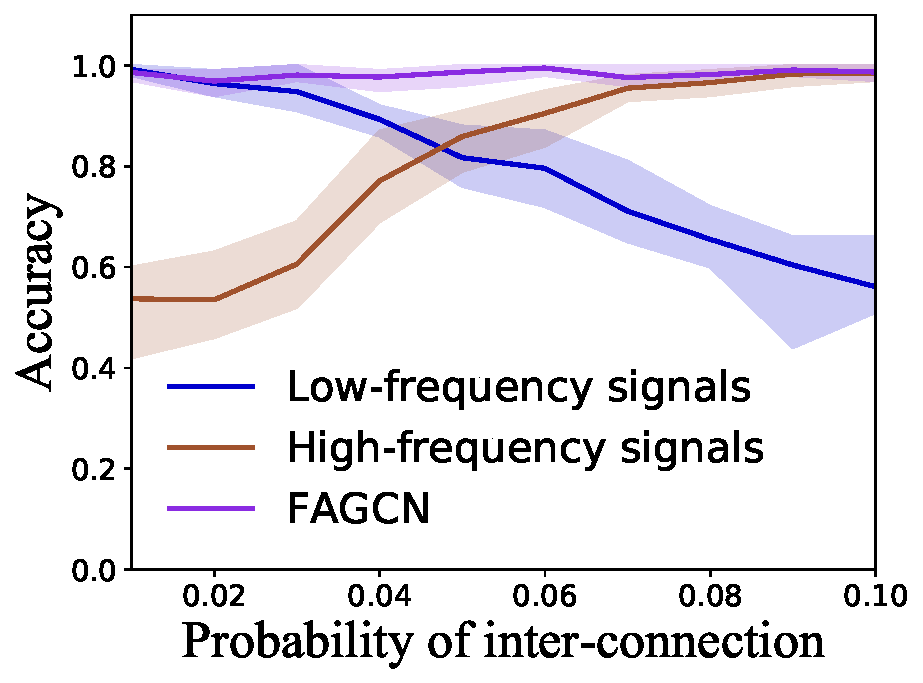
\includegraphics[width=0.31\textwidth]{image/vary_of_q_three}
}
\subfigure[Existing GNNs]{
\label{fig:GNNs}
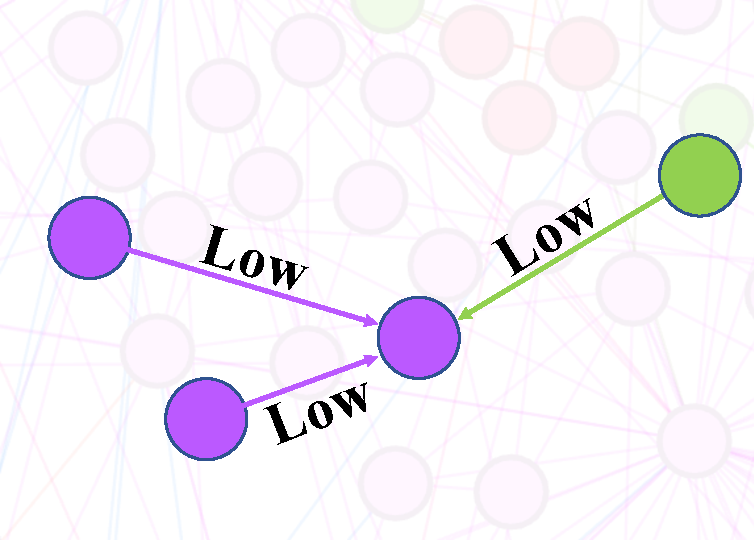
\includegraphics[width=0.31\textwidth]{image/GNN}
}
\subfigure[FAGCN]{
\label{fig:FAGCN}
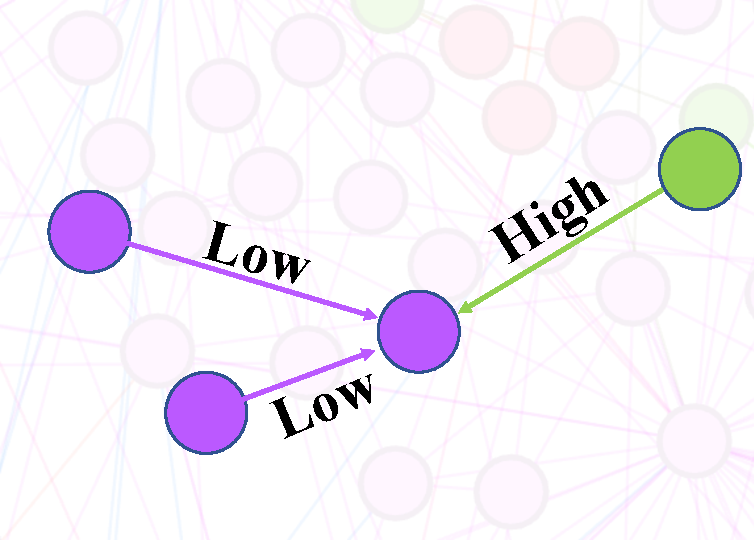
\includegraphics[width=0.31\textwidth]{image/FAGNN}
}
\caption{(a) Classification accuracy of low-frequency signals, high-frequency signals and our model FAGCN. X-axis denotes probability of inter-connection $q$. (b) Existing GNNs aggregate the low-frequency signals of neighbors. (c) FAGCN aggregates the low-frequency signals of neighbors within the same class and high-frequency signals of neighbors from different classes, where the color indicates the node label.}
\label{intro}
\end{figure*}

%Literature has shown that most existing GNNs are essentially low-pass filters \cite{Bridging, SGC}, which preserve the commonalities of node features and reduce the differences among them, thus making the aggregated node representations smooth. This way is effective for assortative networks, i.e., nodes within the same class tend to connect with each other, because the smoothing caused by low-pass filters will make the representations of connected nodes become similar. However, the high-frequency signals, which encode the differences among node features \cite{cvhigh, octave}, are neglected by existing GNNs. \emph{Will high-frequency information in node features also be helpful for GNNs? If so, under what circumstances will the high-frequency signals work?} This is a fundamental question and a well informed answer to this question can help us understand the limitations of GNNs in a principled way.

%As the first contribution of this study, we present experiments assessing the roles of low-frequency and high-frequency signals, where the results clearly show that both of them are helpful for learning node representations (more details are in Section \ref{case}).
%When a network exhibits assortativity, low-frequency signals have good performance, which is consistent with expectations.
%However, when a network exhibits disassortativity, i.e. nodes from different classes tend to connect with each other, high-frequency signals perform much better than low-frequency signals.
%Note that disassortative networks are also ubiquitous, for example, in World Wide Web, there are many hyperlinks connecting different types of web pages \cite{mixing}.

%Once the importance of high-frequency information in GNNs is identified, a natural question is \emph{how to use signals with different frequencies in GNNs?}

To answer this question, two challenges need to be solved:
(1) Both the low-frequency and high-frequency signals are the parts of the raw features. Traditional filter is specifically designed for one certain signal, and cannot well extract different frequency signals  simultaneously.
%there are some complex dependencies among them, which may make them interfere with each other.
(2) Even we can extract different information, however, the assortativity of real-world networks is usually agnostic and varies greatly, moreover, the correlation between task and different information is very complex, so it is difficult to decide what kind of signals should be used: raw features, low-frequency signals, high-frequency signals or their combination.

%The challenges are two-folds: One is how to separate signals with different frequencies. Since the signals in node features are highly coupled, separating the signals of specific frequencies requires careful design.
%Another is how to integrate signals of different frequencies. Because the assortativity of different networks varies greatly and there are multiple signals need to be considered, it is difficult to design a general signal fusion mechanism for different networks.

%how to integrate the low-frequency and high-frequency signals in an effective and efficient way.

%Although GNNs benefit a lot from low-frequency signals \cite{SGC, GraphHeat}, as the network depth increases, their ability to distinguish nodes from different classes decreases \cite{lossexp}.
%On the other hand, high-frequency signals encode the fine details of the network \cite{octave}. The loss of high-frequency information causes a series of problems: over-smoothing \cite{deeper}, reduction of diversity \cite{ramazi2018homophily, recdiversity}, unfairness \cite{karimi2018homophily, fairwalk, Compositional} etc. Therefore, it is important to consider both low-frequency and high-frequency information when designing GNNs.

%that the node representations will maintain low-frequency signals and reduce high-frequency signals through aggregating neighboring features.
%Because low-pass filtering can make the representations of nodes within the same connected component become similar, GNNs can have better performance when the network exhibits homophily, i.e. nodes within the same class tend to connect with each other \cite{revisiting}.

%Although GNNs benefit a lot from low-pass filtering, the loss of high-frequency information leads to the ill presentation of heterophilic nodes, which may cause a series of problems: perception biases \cite{lee2019homophily}, reduction of diversity \cite{ramazi2018homophily, recdiversity} and unfairness \cite{karimi2018homophily, fairwalk, Compositional}. Therefore, it is important to consider both low-frequency and high-frequency information when designing GNNs.

%Therefore, most of the existing GNNs are essentially low-pass filters \cite{Bridging} and the high-frequency signals will reduce a lot after being smoothed by the network structure.

%Despite the loss of high-frequency information, they still have state-of-the-art performance, because the commonly used datasets exhibit homophily, i.e., the number of intra-connection is larger than inter-connection.

%Graph-based abnormal user detection \cite{HACUD, Player2vec, Vendor2vec} aims to utilize the interactions between abnormal users and unlabeled users to detect the potential frauds. However, the potential frauds may try to make deal with the normal users to cover up their intentions. In this situation, the low-frequency signals may fail to find the potential frauds.
%Another example is graph-based recommendation \cite{NGCF, GraphRec}, which treats the aggregation of items as the user's representation and vice versa. Therefore, the frequently purchased items will dominate the user's representation, resulting in the homogenization of the recommendation system, i.e., recommending the similar products to users repeatedly \cite{rechomo}.

In this paper, we design a general frequency adaptation graph convolutional networks called FAGCN, to adaptively aggregate different signals from neighbors or itself.
We first employ the theory of graph signal processing to formally define an enhanced low-pass and high-pass filter to separate the low-frequency and high-frequency signals from the raw features.
Then we design a self-gating mechanism to adaptively integrate the low-frequency signals, high-frequency signals and raw features, without knowing the assortativity of network.
Theoretical analysis proves that FAGCN is a generalization of most existing GNNs and it has a capability to freely shorten or enlarge the distance between node representations, which further explains why FAGCN can perform well on different types of networks.

%and the different signs of edges provide a \emph{cluster property} for the learned representations, i.e. it makes the representations of nodes from the same class similar and nodes of different classes discriminative.
%We theoretically analyze that by setting the edge weights to positive or negative, the local structure becomes either low-pass filter or high-pass filter, which further explains why FAGCN can perform well on different types of networks.

%We theoretically prove that FAGCN is a generalization of most existing GNNs and it provides a \emph{cluster property} for the learned representations, i.e. it makes the representations of nodes from the same class similar and nodes of different classes discriminative.

%In the experiment, we evaluate the performance of our model on two kinds of networks: assortative and disassortative. The results show that FAGCN outperforms most competitive benchmarks on both types of networks. Specially, FAGCN has a large improvement on the disassortative networks.

%Compared with benchmarks, we find that in the homophilic networks, FAGCN makes slightly improvement. On the other hand, compared with state-of-the-art method, FAGCN has a large improvement on heterophilic networks, which proves that FAGCN has more expressive power and performs well on both types of networks.

%: parallelizable, transferable, anisotropic and application to inductive learning.
The contribution of this paper is summarized as follows:
\begin{itemize}
	\item We study the roles of both low-frequency and high-frequency signals in GNNs and verify that high-frequency signals are useful for disassortative networks.
	\item We propose a novel graph convolutional networks FAGCN, which can adaptively change the proportion of low-frequency and high-frequency signals without knowing the types of networks.
	\item We theoretically prove that the expressive power of FAGCN is greater than other GNNs. Moreover, our proposed FAGCN is able to alleviate the over-smoothing problem. Extensive experiments on six real-world networks validate that FAGCN has advantages over state-of-the-arts.
\end{itemize}

\begin{figure*}
\centering
\subfigure[$\mathcal{F}_{L}$]{
\label{low1}
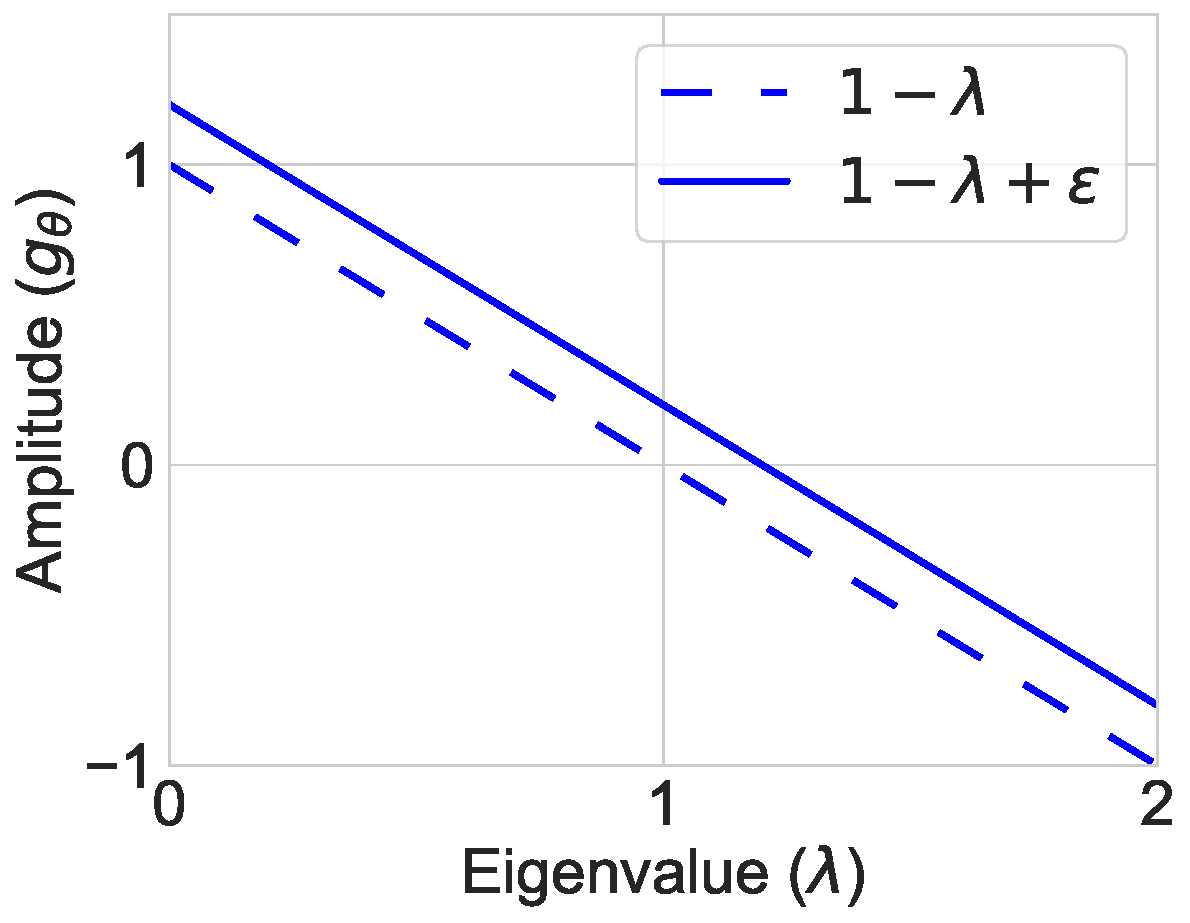
\includegraphics[width=0.23\textwidth]{image/low-1rd}
}
\subfigure[$\mathcal{F}_{L}^{2}$]{
\label{low2}
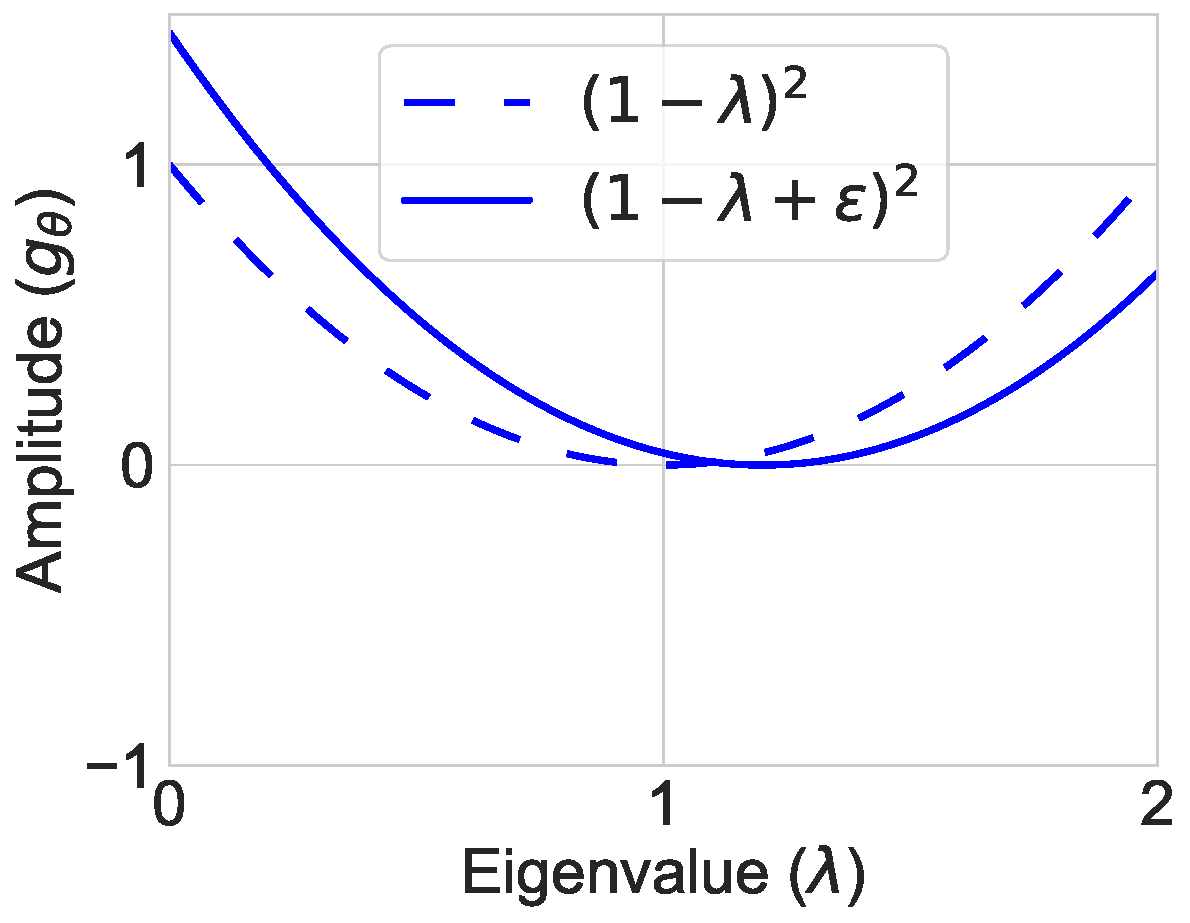
\includegraphics[width=0.23\textwidth]{image/low-2rd}
}
\subfigure[$\mathcal{F}_{H}$]{
\label{high1}
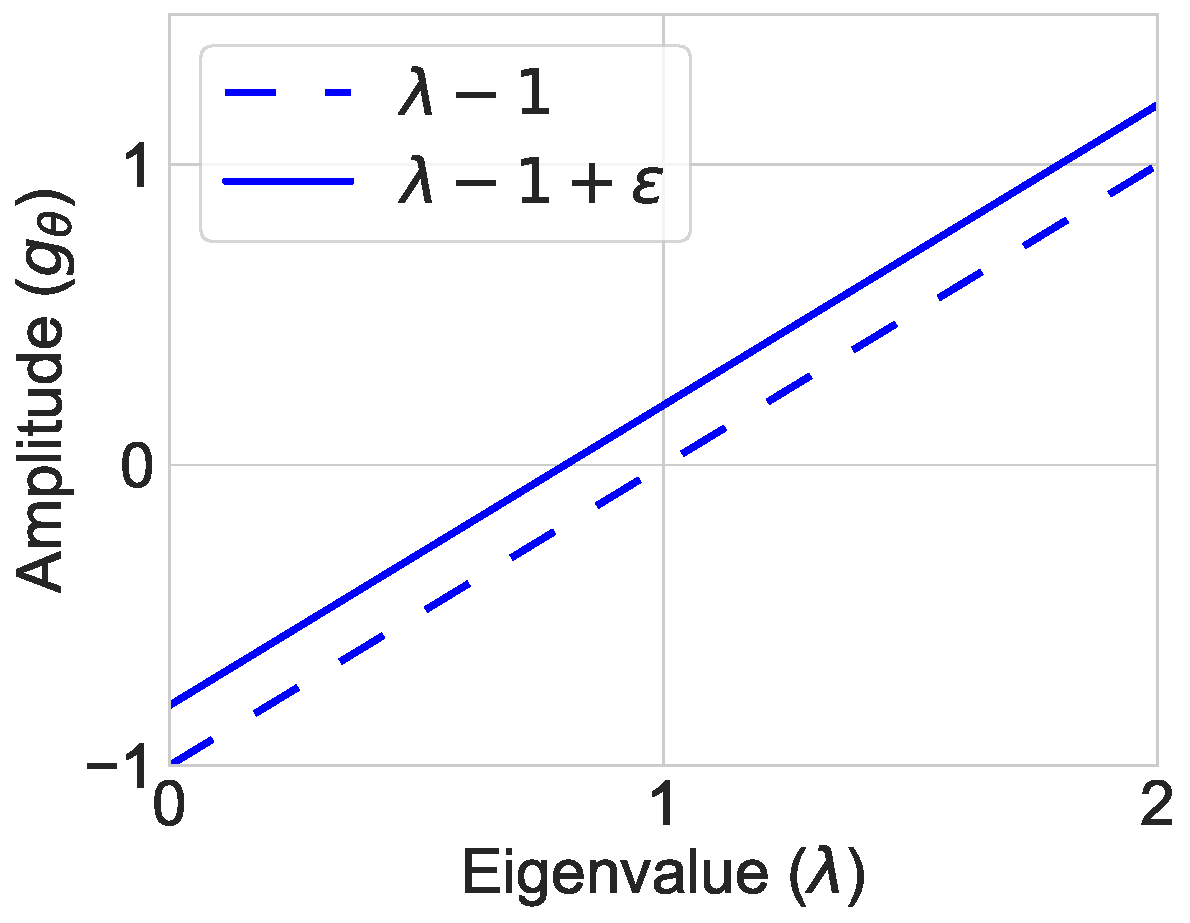
\includegraphics[width=0.23\textwidth]{image/high-1rd}
}
\subfigure[$\mathcal{F}_{H}^{2}$]{
\label{high2}
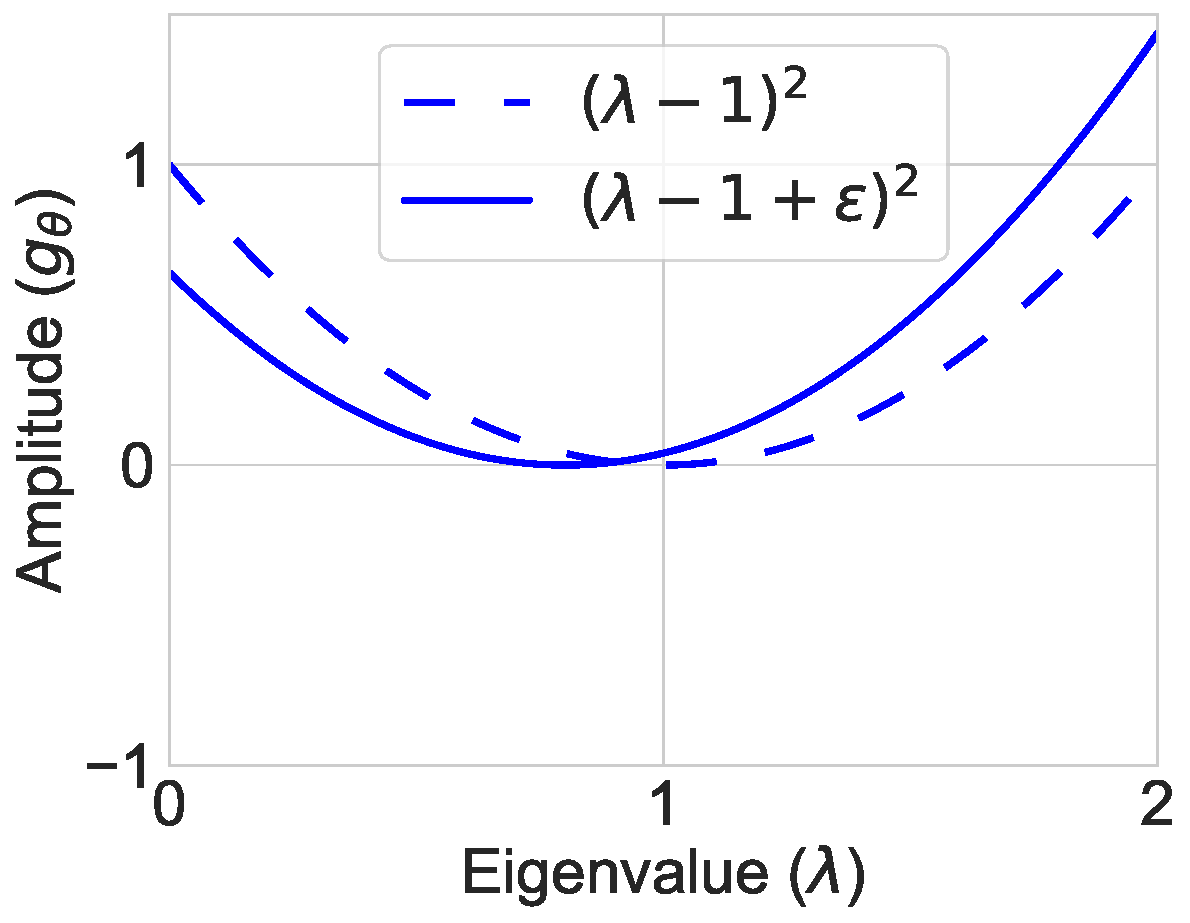
\includegraphics[width=0.23\textwidth]{image/high-2rd}
}
\caption{The relations between eigenvalues and amplitudes in different filters.}
\label{functions}
\end{figure*}

\section{An Experimental Investigation}
\label{case}

In this section, taking the low-frequency and high-frequency signals as an example, we analyze their roles in learning node representations. Specifically, we test their performance of node classification on a series of synthetic networks.
The main idea is to gradually increase the disassortativity of the synthetic networks, and observe how the performance of these two signals changes.
We generate a network with 200 nodes and randomly divide them into 2 classes.
For each node in class one, we sample a 20-dimensional feature vector from Gaussian distribution $\mathcal{N}(0.5,1)$, while for the nodes in class two, the distribution is $\mathcal{N}(-0.5,1)$.
%Besides, we use stochastic blockmodel (SBM) \cite{SBM} to generate network structure conditioned on class labels.
Besides, the connections in the same class are generated from a Bernoulli distribution with probability $p=0.05$, and the probability of connections between two classes $q$ varies from $0.01$ to $0.1$. When $q$ is small, the network exhibits assortativity; As $q$ increases, the network gradually exhibits disassortativity.
We then apply the low-pass and high-pass filters, described in Section \ref{separation}, to node classification task. Half of the nodes are used for training and the remains are used for testing.

Figure \ref{fig:vary_q} illustrates that with the increase of inter-connection $q$, the accuracy of low-frequency signals decreases, while the accuracy of high-frequency signals increases gradually.
This proves that both the low-frequency and high-frequency signals are helpful in learning node representations.
The reason why existing GNNs fail when $q$ increases is that, as shown in Figure \ref{fig:GNNs}, they only aggregate low-frequency signals from neighbors, i.e., making the node representations become similar, regardless of whether nodes belong to the same class, thereby losing the discrimination.
When the network becomes disassortative, the effectiveness of high-frequency signals appears, but as shown in Figure \ref{fig:vary_q}, a single filter cannot achieve optimal results in all cases. Our proposed FAGCN, which combines the advantages of both low-pass and high-pass filters, can aggregate the low-frequency signals of neighbors within the same class and high-frequency signals of neighbors from different classes, as shown in Figure \ref{fig:FAGCN}, thereby showing the best performance on every synthetic network.


\section{Our Proposed Model: FAGCN}
\label{separation}

Consider an undirected graph $G=(V, E)$ with adjacency matrix $A \in \mathbb{R}^{N \times N}$, where $V$ is a set of nodes with $\left| V \right| = N$ and $E$ is a set of edges. The normalized graph Laplacian matrix is defined as $L=I_{n}-D^{-1/2}AD^{-1/2}$, where $D \in \mathbb{R}^{N \times N}$ is a diagonal degree matrix with $D_{i,i}=\sum_{j}A_{i,j}$ and $I_{n}$ denotes the identity matrix. Because $L$ is a real symmetric matrix, it has a complete set of orthonormal eigenvectors $\{u_{l}\}_{l=1}^{n} \in \mathbb{R}^{n}$, each of which has a corresponding eigenvalue $\lambda_{l} \in [0, 2]$ \cite{spectralgraph}. Through the eigenvalues and eigenvectors, we have $L=U\Lambda U^{\top}$, where $\Lambda=diag([ \lambda_{1},\lambda_{2},\cdots,\lambda_{n} ])$.

\textbf{Graph Fourier Transform.}
According to theory of graph signal processing \cite{GSP}, we can treat the eigenvectors of normalized Laplacian matrix as the bases in graph Fourier transform. Given a signal $x \in \mathbb{R}^{n}$, the graph Fourier transform is defined as $\hat{x}=U^{\top}x$, and the inverse graph Fourier transform is $x=U\hat{x}$. Thus, the convolutional $*_{G}$ between the signal $x$ and convolution kernel $f$ is:
\begin{equation}
\label{convolution}
	f *_{G} x = U \left( \left( U^{\top}f \right) \odot \left( U^{\top}x \right) \right) = Ug_{\theta}U^{\top}x,
\end{equation}
where $\odot$ denotes the element-wise product of vectors and $g_{\theta}$ is a diagonal matrix, which represents the convolutional kernel in the spectral domain, replacing $U^{\top}f$. Spectral CNN \cite{SpectralCNN} uses a non-parametric convolutional kernel $g_{\theta}=diag(\{ \theta_{i} \}_{i=1}^{n})$. ChebNet \cite{ChebNet} parameterizes convolutional kernel with a polynomial expansion $g_{\theta}=\sum_{k=0}^{K-1}\alpha_{k}\Lambda^{k}$. GCN defines the convolutional kernel as $g_{\theta}=I-\Lambda$.

\subsection{Separation}
As discussed in Section \ref{case}, both the low-frequency and high-frequency signals are helpful for learning node representations.
To make full use of them, we design a low-pass filter $\mathcal{F}_{L}$ and a high-pass filter $\mathcal{F}_{H}$ to separate the low-frequency and high-frequency signals from the node features:
\begin{gather}
	\mathcal{F}_{L} = \varepsilon I + D^{-1/2}AD^{-1/2} = (\varepsilon+1) I - L, \notag \\
	\mathcal{F}_{H} = \varepsilon I - D^{-1/2}AD^{-1/2} = (\varepsilon-1) I + L, \label{filters}
\end{gather}
where $\varepsilon$ is a scaling hyper-parameter limited in $[0, 1]$. If we use $\mathcal{F}_{L}$ and $\mathcal{F}_{H}$ to replace the convolutional kernel $f$ in Equation \ref{convolution}. The signal $x$ is filtered by $\mathcal{F}_{L}$ and $\mathcal{F}_{H}$ as:
\begin{gather}
	\mathcal{F}_{L} *_{G} x = U[(\varepsilon+1) I - \Lambda]U^{\top}x = \mathcal{F}_{L} \cdot x, \notag \\
	\mathcal{F}_{H} *_{G} x = U[(\varepsilon-1) I + \Lambda]U^{\top}x = \mathcal{F}_{H} \cdot x.
	\label{filterings}
\end{gather}
Therefore, the convolutional kernel of $\mathcal{F}_{L}$ is $g_{\theta}=(\varepsilon+1) I - \Lambda$, rewritten as $g_{\theta}(\lambda_{i})=\varepsilon+1-\lambda_{i}$, shown in Figure \ref{low1}. When $\lambda_{i} > 1+\varepsilon$, $g_{\theta}(\lambda_{i}) < 0$, which gives a negative amplitude.
To avoid this, we consider the second-order convolution kernel $\mathcal{F}_{L}^{2}$ with $g_{\theta}(\lambda_{i})=(\varepsilon+1-\lambda_{i})^{2}$, shown in Figure \ref{low2}. When $\lambda_{i} = 0$, $g_{\theta}(\lambda_{i}) = (\varepsilon+1)^{2} > 1$ and when $\lambda_{i} = 2$, $g_{\theta}(\lambda_{i}) = (\varepsilon-1)^{2} < 1$, which amplifies the low-frequency signals and restrains the high-frequency signals.
%The same for the analysis of $\mathcal{F}_{H}$ and $\mathcal{F}_{H}^{2}$ in Figure \ref{high1} and \ref{high2}.
\begin{remark}
	(Enhanced filters) As in Figure \ref{functions}, compared with traditional low-pass filters, e.g., GCN and SGC \cite{SGC}, $\mathcal{F}_{L}$ is an enhanced low-pass filter. Convolutional kernel of second-order GCN is $g_{\theta}(\lambda_{i})=(1-\lambda_{i})^{2}$. When $\lambda_{i}=0$, the amplitude of GCN is $g_{\theta}(\lambda_{i})=1<(1+\varepsilon)^{2}$. Hence, the value of $\mathcal{F}_{L}$ is greater than GCN in low-pass filtering. Similarly, $\mathcal{F}_{H}$ is an enhanced high-pass filter, which provides a greater value for the high-frequency signals.
\end{remark}

Separating the low-frequency and high-frequency signals from the node features provides a feasible way to deal with different networks, e.g., low-frequency signals for assortative networks and high-frequency signals for disassortative networks.
However, this way has two disadvantages: One is that selecting signals requires a priori knowledge, i.e., we actually do not know whether a network is assortative or disassortative beforehand. The other is that, as in Equation \ref{filterings}, it requires matrix multiplication, which is undesirable for large graphs \cite{GraphSAGE}.
Therefore, an efficient method that can adaptively aggregate low-frequency and high-frequency signals is desired.

%\begin{figure*}
%\centering
%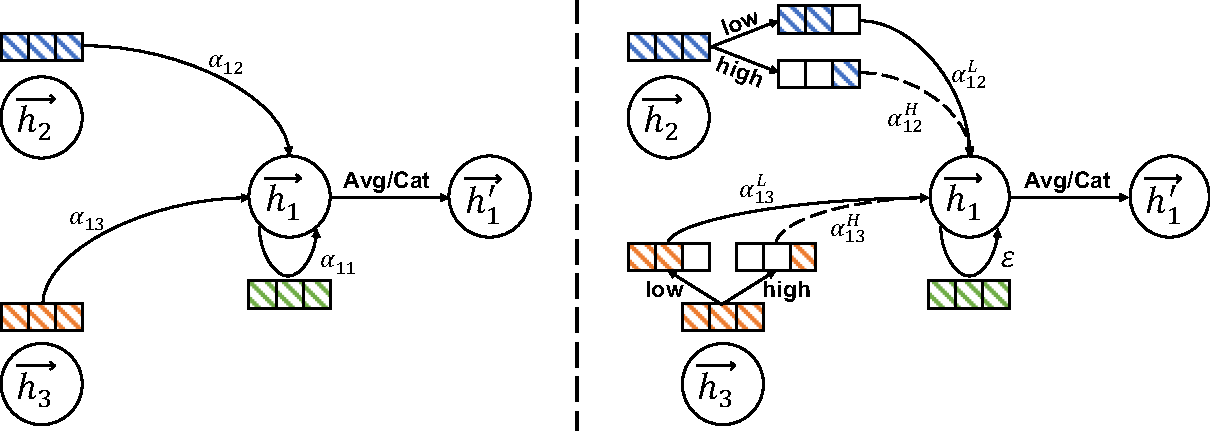
\includegraphics[width=0.95\linewidth]{image/model}
%\caption{\textbf{Left:} The aggregation process of existing GNNs, and $\alpha_{ij}$ indicates the importance of node $j$ to node $i$. \textbf{Right:} The aggregation process of FAGCN, and $\alpha_{ij}^{L}$, $\alpha_{ij}^{H}$ denote the proportions of low-frequency and high-frequency signals of node $j$ to node $i$, respectively.}
%\label{model}
%\end{figure*}

\begin{remark}
\label{rema}
	(Concrete meaning of signals)
	In Equation \ref{filters}, we have $\mathcal{F}_{L} = \varepsilon I + D^{-1/2}AD^{-1/2}$ and $\mathcal{F}_{H} = \varepsilon I - D^{-1/2}AD^{-1/2}$.
	Therefore, the concrete meaning of low-frequency signal $\mathcal{F}_{L} \cdot x$ is the sum of node features and neighborhood features in spatial domain, while high-frequency signal $\mathcal{F}_{H} \cdot x$ represents the difference between node features and neighborhood features in spatial domain.
\end{remark}

\begin{figure}
\centering
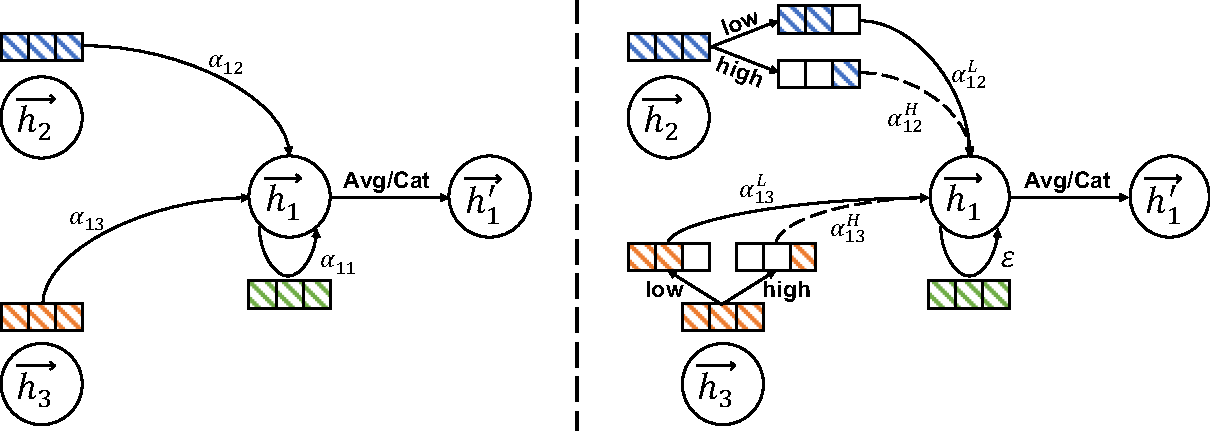
\includegraphics[width=\linewidth]{image/model}
\caption{\textbf{Left:} The aggregation process of existing GNNs, and $\alpha_{ij}$ indicates the importance of node $j$ to node $i$. \textbf{Right:} The aggregation process of FAGCN, and $\alpha_{ij}^{L}$, $\alpha_{ij}^{H}$ denote the proportions of low-frequency and high-frequency signals of node $j$ to node $i$, respectively.}
\label{model}
\end{figure}

\subsection{Aggregation}
Before introducing the details, we first compare the aggregation process of existing GNNs and FAGCN in Figure \ref{model}. The left shows that existing GNNs consider learning the importance ($\alpha_{ij}$) of each node in aggregation. The right is FAGCN that uses two coefficients ($\alpha^{L}_{ij}$ and $\alpha^{H}_{ij}$) to aggregate low-frequency and high-frequency signals from the neighbors, respectively.

The input of our model are the node features, $\mathbf{H}=\{ \mathbf{h}_{1},\mathbf{h}_{2},\cdots,\mathbf{h}_{N} \} \in \mathbb{R}^{N \times F}$, where $F$ is the dimension of the node features.
For the purpose of frequency adaptation, a basic idea is to use the attention mechanism to learn the proportion of low-frequency and high-frequency signals:
\begin{equation}
	\tilde{\mathbf{h}}_{i} = \alpha_{ij}^{L} (\mathcal{F}_{L} \cdot \mathbf{H})_{i} + \alpha_{ij}^{H} (\mathcal{F}_{H} \cdot \mathbf{H})_{i} = \varepsilon \mathbf{h}_{i} + \sum_{j \in \mathcal{N}_{i}} \frac{\alpha_{ij}^{L} - \alpha_{ij}^{H}}{\sqrt{d_{i}d_{j}}} \mathbf{h}_{j},
\end{equation}
where $\tilde{\mathbf{h}}_{i}$ is the aggregated representation of node $i$. $\mathcal{N}_{i}$ and $d_{i}$ denote the neighbor set and degree of node $i$, respectively. $\alpha_{ij}^{L}$ and $\alpha_{ij}^{H}$ represent the proportions of node $j$'s low-frequency and high-frequency signals to node $i$.
We set $\alpha_{ij}^{L} + \alpha_{ij}^{H}=1$ and $\alpha_{ij}^{G} = \alpha_{ij}^{L} - \alpha_{ij}^{H}$.
In the following, we show that $\alpha_{ij}^{G}$ can be interpreted from two perspectives.

\begin{remark}
	(Two perspectives of $\alpha_{ij}^{G}$) One is that $\alpha_{ij}^{G}$ indirectly represents the proportion of low-frequency and high-frequency signals.  $\alpha_{ij}^{G} > 0$, i.e., $\alpha_{ij}^{L} > \alpha_{ij}^{H}$, means that low-frequency signals dominate the representations and vice versa.
	Based on $\alpha_{ij}^{G}$, we can calculate the value of $\alpha_{ij}^{L}$ and $\alpha_{ij}^{H}$, so as to achieve the proportions of signals.
	Another is that $\alpha_{ij}^{G}$ denotes the coefficients of neighbors in aggregation. $\alpha_{ij}^{G} > 0$ represents the sum of node features and neighborhood features, i.e., $\mathbf{h}_{i} + \mathbf{h}_{j}$, while $\alpha_{ij}^{G} < 0$ represents the difference between them, i.e., $\mathbf{h}_{i} - \mathbf{h}_{j}$, as explained in Remark \ref{rema}. Besides, when $\alpha_{ij}^{G} \approx 0$, the contributions of neighbors will be limited, so the raw features will dominate the node representations.
%	This maybe useful when the network is heavily disassortative.
\end{remark}

In order to learn the coefficients $\alpha_{ij}^{G}$ effectively, we need to consider the features of both the node itself and its neighbors.
%Similar to the self-attention mechanism \cite{Transformer} that assigns different transformations for `query', `key' and `value', we use two shared weight matrices $\mathbf{W}_{q}, \mathbf{W}_{v} \in \mathbb{R}^{F' \times F}$ to transform the node features into query space and value space, respectively.
Therefore, we propose a shared \emph{self-gating} mechanism $\mathbb{R}^{F} \times \mathbb{R}^{F} \to \mathbb{R}$ to learn the coefficients:
\begin{equation}
\label{tanh}
	\alpha_{ij}^{G}=\tanh \left( \mathbf{g}^{\top} \left[ \mathbf{h}_{i} \parallel \mathbf{h}_{j} \right] \right),
\end{equation}
where $\parallel$ denotes the concatenation operation, $\mathbf{g} \in \mathbb{R}^{2F}$ can be seen as a shared convolutional kernel \cite{GAT} and $\tanh(\cdot)$ is the hyperbolic tangent function, which can naturally limits the value of $\alpha_{ij}^{G}$ in $[-1, 1]$. Besides, to make use of the structural information, we only calculate the coefficients among the node and its first-order neighbors $\mathcal{N}_{i}$.

After calculating $\alpha_{ij}^{G}$, we can aggregate the representations of neighbors:
\begin{equation}
\label{self-gating}
	\mathbf{h}_{i}^{'}= \varepsilon \mathbf{h}_{i} + \sum_{j \in \mathcal{N}_{i}} \frac{\alpha_{ij}^{G}}{\sqrt{d_{i}d_{j}}} \mathbf{h}_{j},
\end{equation}
where $\mathbf{h}_{i}^{'}$ denotes the aggregated representation of node $i$. Note that when aggregating information from neighbors, the degrees are used to normalize the coefficients, thus preventing the aggregated representations from being too large.
%Furthermore, to reduce variance and make the model capture the information from different aspects \cite{Transformer}, we extend the self-gating to \emph{multi-head gating}, which concatenates or averages the aggregated representations from $K$ aspects:
%\begin{equation}
%	\mathbf{h}_{i}^{'}=\mathop{\parallel}\limits_{k=1}^{K} \phi \left( \varepsilon \mathbf{W}_{v}^{k} \mathbf{h}_{i} + \sum_{j \in \mathcal{N}_{i}} \frac{\alpha_{ij}^{G^{k}}}{\sqrt{d_{i}d_{j}}} \mathbf{W}_{v}^{k} \mathbf{h}_{j} \right).
%\end{equation}
\subsection{The Whole Architecture of FAGCN}
In the previous section, we introduce the message passing process of FAGCN. Here, we formally define the whole architecture of FAGCN. Some recent studies \cite{SGC, cui2020adaptive} emphasize that the entanglement of filters and weight matrices may be harmful to the performance and robustness of the model. Motivated by this, we first use a multilayer perceptron (MLP) to apply the non-linear transform to the raw features. Then we propagate the representations through Eq. \ref{self-gating}. The mathematical expression of FAGCN is defined as:
\begin{align}
    \mathbf{h}^{(0)}_{i} & = \phi(\mathbf{W}_{1}\mathbf{h}_{i}) & \in \mathbb{R}^{F' \times 1} \notag \\
    \mathbf{h}^{(l)}_{i} & = \varepsilon \mathbf{h}^{(0)}_{i} + \sum_{j \in \mathcal{N}_{i}} \frac{\alpha_{ij}^{G}}{\sqrt{d_{i}d_{j}}} \mathbf{h}^{(l-1)}_{j} & \in \mathbb{R}^{F' \times 1} \notag \\
    \mathbf{h}_{out} & = \mathbf{W}_{2}\mathbf{h}^{(L)}_{i} & \in \mathbb{R}^{K \times 1},
\end{align}
where $\mathbf{W}_{1} \in \mathbb{R}^{F \times F'}, \mathbf{W}_{2} \in \mathbb{R}^{F' \times K}$ are the weight matrices, $\phi$ is the activation function, $F^{'}$ denotes the dimension of hidden layers, $l$ indicates the layers, ranging from 1 to $L$, and $K$ represents the number of classes.
The complexity of a single layer FAGCN is $\mathcal{O}((N + |E|) \times F')$, which is approximately linear with the number of edges and nodes.

\section{Theoretical Analysis}
\label{theory}

\subsection{Connection to Existing GNNs}

FAGCN is a generalization of most existing GNNs. Specifically, when we set the coefficients $\alpha_{ij}^{G}$ to 1, FAGCN acts like GCN and when we use softmax function to normalize $\alpha_{ij}^{G}$, FAGCN becomes GAT.
Therefore, as indicated in Remark \ref{rema}, because the coefficients in GCN and GAT are both greater than zero, they prefer to aggregate the low-frequency signals. However, FAGCN can learn a coefficient that can be positive or negative, to adaptively aggregate low-frequency and high-frequency signals.

\subsection{Expressive Power of FAGCN}
\label{sec:expressive}

We analyze the expressive power of FAGCN from the perspective of the distance between node representations.
Assume that $(u, v)$ is a pair of connected nodes, and $\mathbf{h}_{u}, \mathbf{h}_{v}$ are the node features. Let $\mathcal{D}, \mathcal{D}_{L}, \mathcal{D}_{H}$ be the distance of node features, low-frequency signals of node features and high-frequency signals of node features, respectively.
\begin{align}
	\mathcal{D} = \| \mathbf{h}_{u}-\mathbf{h}_{v} \|_{2}. \notag \\
	\mathcal{D}_{L} = \| (\varepsilon\mathbf{h}_{u}+\mathbf{h}_{v}) - (\varepsilon\mathbf{h}_{v}+\mathbf{h}_{u}) \|_{2} &= | 1-\varepsilon |\mathcal{D}. \notag \\
	\mathcal{D}_{H} = \| (\varepsilon\mathbf{h}_{u}-\mathbf{h}_{v}) - (\varepsilon\mathbf{h}_{v}-\mathbf{h}_{u}) \|_{2} &= | 1+\varepsilon |\mathcal{D}. \notag
\end{align}

%\begin{gather}
%	\mathcal{D} = \| \mathbf{h}_{u}-\mathbf{h}_{v} \|_{2}. \notag \\
%	\mathcal{D}_{L} = \| (\varepsilon\mathbf{h}_{u}+\mathbf{h}_{v}) - (\varepsilon\mathbf{h}_{v}+\mathbf{h}_{u}) \|_{2} &= \| (1-\varepsilon)\mathbf{h}_{v} - (1-\varepsilon)\mathbf{h}_{u} \|_{2}=| 1-\varepsilon |\mathcal{D}. \notag \\
%	\mathcal{D}_{H} = \| (\varepsilon\mathbf{h}_{u}-\mathbf{h}_{v}) - (\varepsilon\mathbf{h}_{v}-\mathbf{h}_{u}) \|_{2} &= \| (1+\varepsilon)\mathbf{h}_{u} - (1+\varepsilon)\mathbf{h}_{v} \|_{2}=| 1+\varepsilon |\mathcal{D}. \notag
%\end{gather}

\begin{proposition}
\label{prop1}
	Low-pass filtering makes the representations become similar, while high-pass filtering makes the representations become discriminative.
\end{proposition}

\begin{proof}
	It is easy to see that $\mathcal{D}_{H} > \mathcal{D} > \mathcal{D}_{L}$.
	This indicates that compared with the original distance $\mathcal{D}$, the distance $\mathcal{D}_{L}$ induced by low-frequency signals is smaller, implying that low-frequency signals can make the representations of connected nodes become similar.
	While the distance $\mathcal{D}_{H}$ induced by high-frequency signals is larger, implying that high-frequency signals can make the representations of connected nodes become discriminative.
\end{proof}

We have analyzed the roles of low-frequency and high-frequency signals in representation learning. Obviously, FAGCN can choose to shorten or enlarge the distance between node representations flexibly, while most existing GNNs cannot.

\begin{proposition}
	Most existing GNNs, e.g., GCN, only have the capability to make representations of nodes become similar.
\end{proposition}

\begin{proof}
	The filter used in GCN is: $(D+I)^{-1/2}(A+I)(D+I)^{-1/2}$.
	Hence, the distance of representations learned by GCN is: $\mathcal{D}_{G} \approx \| (\frac{1}{d_{u}} \mathbf{h}_{u} + \mathbf{h}_{v}) - (\frac{1}{d_{v}} \mathbf{h}_{v} + \mathbf{h}_{u}) \|_{2} \approx |1-\frac{1}{d}|\mathcal{D} < \mathcal{D}$ (s.t. $d_{u} \approx d_{v} \approx d$).
\end{proof}

%It can be seen that GCN will shorten the distance of two connected nodes, which may cause over-smoothing \cite{deeper}.

%\begin{hypothesis}
%\label{hypo}
%	Equation \ref{tanh} is likely to have the capability that when $u$ and $v$ belong to the same class, it outputs $\alpha_{uv}^{G} \approx \alpha_{vu}^{G} \approx 1$, so that FAGCN can aggregate the low-frequency from the neighbors in the same class.
%	When $u$ and $v$ belong to different classes, it outputs $\alpha_{uv}^{G} \approx \alpha_{vu}^{G} \approx -1$. In this way, high-frequency signals will dominate the representations of neighbors from different classes.
%\end{hypothesis}
%
%Through the case study in Section \ref{case}, we can speculate that Equation \ref{tanh} has the capability to distinguish whether two nodes belong to same class. And it will help FAGCN to aggregate the low-frequency signals from nodes within the same class and high-frequency signals of nodes from different classes. In Section \ref{visualexperiment}, we use the visualization of coefficients to verify this hypothesis. Based on this hypothesis, we further prove that FAGCN has a capability called \emph{cluster property}.
%
%\begin{proposition}
%\label{prop2}
%	(cluster property)
%	The representations learned by FAGCN possesses the clustering property, i.e., representations of nodes within the same class are similar and nodes from different classes are discriminative.
%\end{proposition}
%
%\begin{proof}
%	The distance of representations learned by FAGCN can be defined as:
%	\begin{equation}
%		\mathcal{D}_{F}=\left \| (\varepsilon \mathbf{h}_{u} + \alpha_{uv}^{G} \mathbf{h}_{v}) - (\varepsilon \mathbf{h}_{v} + \alpha_{vu}^{G}  \mathbf{h}_{u}) \right \|_{2}. \notag
%	\end{equation}
%	According to Hypothesis \ref{hypo}, if $u$ and $v$ belong to the same class, $\alpha_{uv}^{G} \approx \alpha_{vu}^{G} \approx 1$. Hence, $\mathcal{D}_{F} \approx \mathcal{D}_{L}$ and FAGCN acts as a low-pass filter. According to Proposition \ref{prop1}, FAGCN will make the representations become similar. When $u$ and $v$ belong to different classes, $\alpha_{uv}^{G} \approx \alpha_{vu}^{G} \approx -1$, $\mathcal{D}_{F} \approx \mathcal{D}_{H}$, FAGCN acts as a high-pass filter, making the representations become discriminative.
%\end{proof}

\section{Experiments}
%We evaluate the performance of FAGCN on two kinds of datasets (assortative as well as disassortative), by comparing with a series of strong benchmarks. Section \ref{datasets} and Section \ref{setup} summarize the details of datasets and experimental setup. And we make some quantitative and qualitative experiments to prove the superiority of our model compared with the existing GNNs.

\subsection{Datasets}
\label{datasets}

\begin{table}
  \centering
  \caption{The statistics of datasets}
	\resizebox{\linewidth}{!}{
    \begin{tabular}{lcrrrrr}
    \toprule
    \textbf{Dataset} & \textbf{Assortivity} & \textbf{Nodes} & \textbf{Edges} & \textbf{Classes} & \textbf{Features} \\
    \midrule
    Cora  & 0.771 & 2,708 & 5,429 & 7 & 1,433 \\
    Citeseer & 0.671 & 3,327 & 4,732 & 6 & 3,703 \\
    Pubmed & 0.686 & 19,717 & 44,338 & 3 & 500	\\
	\midrule
%    Cornell & Entangled & 183   & 295   & 5     & 1,703	& 0.25 \\
%    Texas & Entangled & 183   & 309   & 5     & 1,703	& 0.22 \\
%    Wisconsin & Entangled & 251   & 499   & 5     & 1,703	& 0.24 \\
    Chameleon	& 0.180 & 2,277 & 36,101 & 3 & 2,325 \\
    Squirrel	& 0.018 & 5,201 & 217,073 & 3 & 2,089 \\
    Actor		& 0.003 & 7,600 & 33,544 & 5 & 931	\\
%    Cornell		& - & 183 & 295 & 5 & 1,703\\
%    Texas		& - & 183 & 309 & 5 & 1,703\\
%    Wisconsin	& - & 251 & 	499 & 5 & 1,703\\
    \bottomrule
    \end{tabular}}
\label{statistic}
\end{table}

\begin{figure*}
\centering
\subfigure[Chameleon]{
\label{Chameleon}
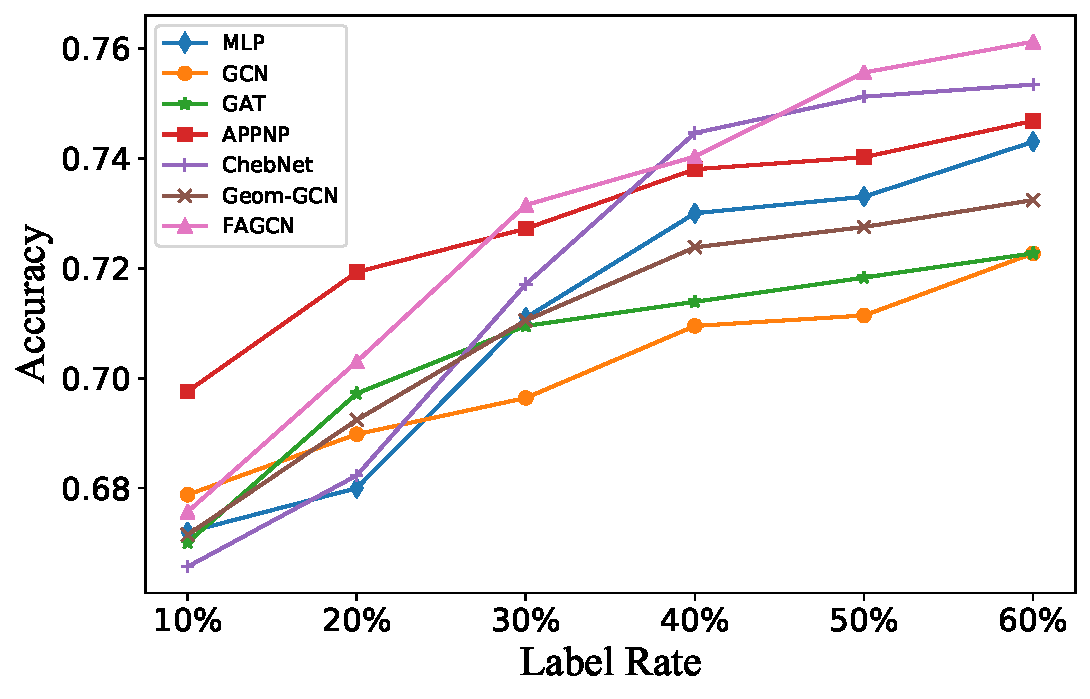
\includegraphics[width=0.31\textwidth]{image/Chameleon}
}
\subfigure[Squirrel]{
\label{Squirrel}
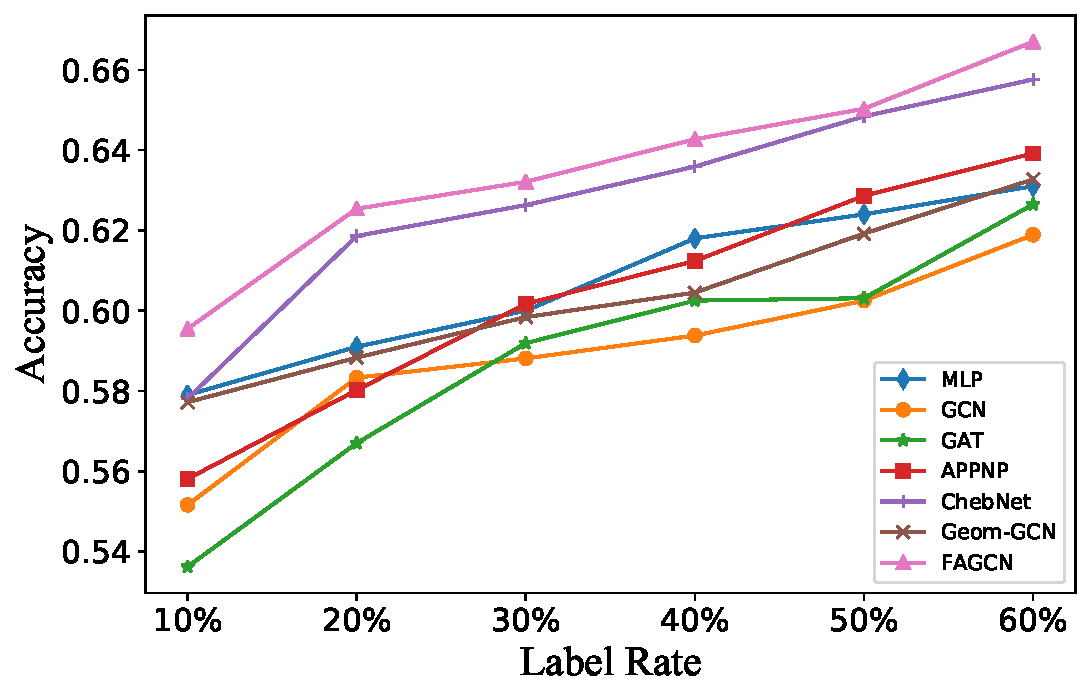
\includegraphics[width=0.31\textwidth]{image/Squirrel}
}
\subfigure[Actor]{
\label{Actor}
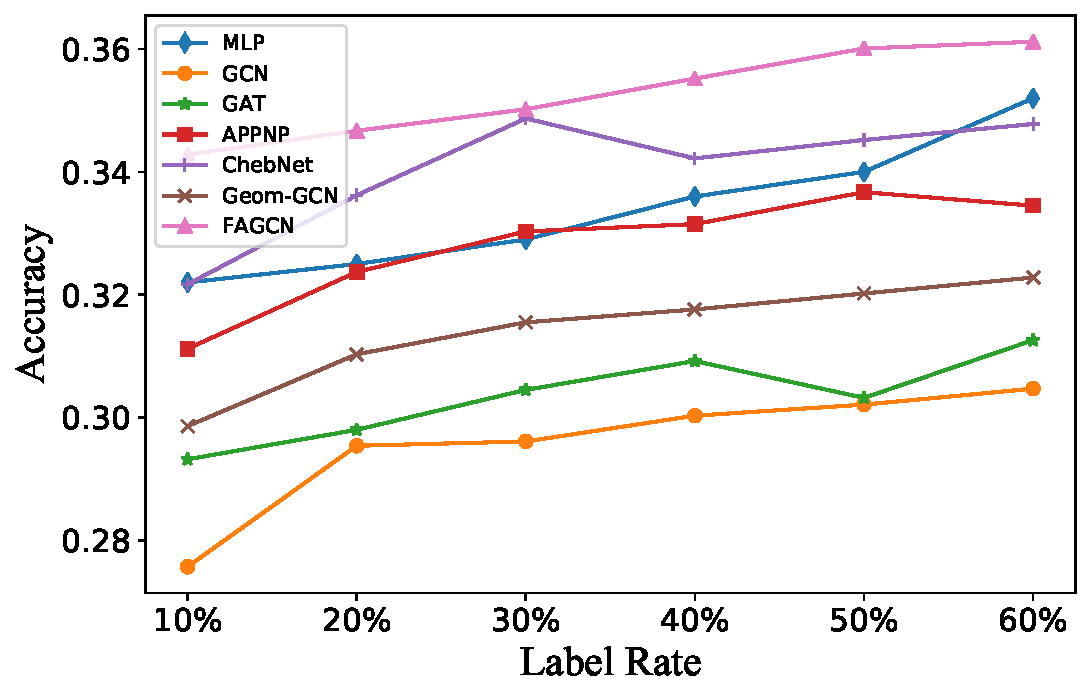
\includegraphics[width=0.31\textwidth]{image/Actor}
}
\caption{Classification accuracy of different methods under different label rates on disassortative networks.}
\label{disassortative}
\end{figure*}

\textbf{Assortative datasets.} We choose the commonly used \emph{citation networks}, e.g., Cora, Citeseer and Pubmed for assortative datasets. Edges in these networks represent the citation relationship between two papers (undirected), node features are the bag-of-words vector of the papers and labels are the fields of papers. In each network, we use 20 labeled nodes per class for training, 500 nodes for validation and 1000 nodes for testing. Details can be found in \cite{GCN}.

\noindent
\textbf{Disassortative datasets.} We consider the \emph{Wikipedia networks}\footnote{http://snap.stanford.edu/data/wikipedia-article-networks.html} and \emph{Actor co-occurrence network} \cite{actornet} for disassortative datasets.
Chameleon and Squirrel are two Wikipedia networks. Edges represent the hyperlinks between two pages, node features are some informative nouns in the pages and labels correspond to the traffic of the pages.
In Actor co-occurrence network, each node represents an actor, and the edges denote the collaborations of them. Node features are the keywords in Wikipedia and labels are the types of actors.
%Cornell, Texas and Wisconsin are three webpage networks, collected by Carnegie Mellon University. Each node is a webpage and edges represent the hyperlinks between them. Node features are the bag-of-words of webpages and labels are the types of webpages.
Since there is no standard division for these networks. To verify the effectiveness and robustness, we use 20\% for validation, 20\% for testing and change the training ratio from 10\% to 60\%.

More detailed characteristics of the datasets can be found in Table \ref{statistic}. Note that a higher value of the second column represents a more obvious assortativity \cite{mixing}.

\subsection{Experimental Setup}
\label{setup}

We compare FAGCN with two types of representative GNNs: Spectral-based methods, i.e., SGC \cite{SGC},  GCN \cite{GCN}, ChebNet \cite{ChebNet} and GWNN \cite{GWNN}; Spatial-based methods, i.e., GIN \cite{GIN}, GAT \cite{GAT}, MoNet \cite{MoNet}, GraphSAGE \cite{GraphSAGE} and APPNP \cite{PPNP}. For disassortative networks, we add Geom-GCN \cite{GeomGCN} and MLP as new benchmarks.
All methods were implemented in Pytorch with Adam optimizer \cite{Adam}.
%For each method, we apply a two-layer model for node classification task with ELU activation function \cite{ELU} for GAT and ReLU \cite{ReLU} for others.
We run 10 times and report the mean values with standard deviation. The hidden unit is fixed at 16 in assortative networks and 32 in disassortative networks.
The hyper-parameter search space is: learning rate in \{0.01, 0.005\}, dropout in \{0.4, 0.5, 0.6\}, weight decay in \{1$E$-3, 5$E$-4, 5$E$-5\}, number of layers in \{1, 2, $\cdots$, 8\}, $\varepsilon$ in \{0.1, $\cdots$, 1.0\}.

In assortative datasets, we use hyper-parameters in previous literature for baselines. For FAGCN, the hyper-parameter setting is: learning rate = 0.01, dropout = 0.6, weight decay = 1$E$-3, layers = 4. $\varepsilon$ = 0.2, 0.3, 0.3 for Cora, Citeseer and Pubmed. The patience of early stop is set to 100.
In disassortative datasets, the hyper-parameter for FAGCN is: learning rate = 0.01, dropout = 0.5, weight decay = 5$E$-5, layers = 2. $\varepsilon$ = 0.4, 0.3, 0.5 for Chameleon, Squirrel and Actor, respectively.
Besides, we run 500 epochs and choose the model with highest validation accuracy for testing.

\subsection{Classification on Different Types of Networks}
\label{sec:results}

\newsavebox{\tablebox}
\begin{table}
  \centering
  \caption{Summary of node classification results (in percent).}
	\begin{lrbox}{\tablebox}
    \begin{tabular}{lcccccc}
    \toprule
    \textbf{Method} & \textbf{Cora} & \textbf{Citeseer} & \textbf{Pubmed} \\
    \midrule
	SGC & 81.0\% & 71.9\% & 78.9\% \\
    GCN & 81.5\% & 70.3\% & 79.0\% \\
    GWNN & 82.8\% & 71.7\% & 79.1\%\\
    ChebNet & 81.2\% & 69.8\% & 74.4\%\\
    GraphHeat & 83.7\% & 72.5\% & \textbf{80.5\%}\\
	\midrule
	GIN & 77.6\% & 66.1\% & 77.0\%\\
	GAT & 83.0\% & 72.5\% & 79.0\%\\
	MoNet & 81.7\% & -     & 78.8\%\\
	APPNP & 83.7\% & 72.1\% & 79.2\%\\
    GraphSAGE & 82.3\% & 71.2\% & 78.5\%\\
    \midrule
%    FAGCN (rand. splits) & - & - & - & 78.82$\pm$1.78 & 44.9$\pm$1.7 & 36.1$\pm$0.4 \\
%    FAGCN-2 & 83.6$\pm$0.3\% & 71.5$\pm$0.5\% & 79.4$\pm$0.3\%\\
	\textbf{FAGCN} & \textbf{84.1$\pm$0.5\%} & \textbf{72.7$\pm$0.8\%} & 79.4$\pm$0.3\% \\
    \bottomrule
    \end{tabular}
    \end{lrbox}
    \scalebox{1}{\usebox{\tablebox}}
  \label{assortative}
\end{table}


\begin{figure}[t]
    \centering
    \subfigure[Cora]{
        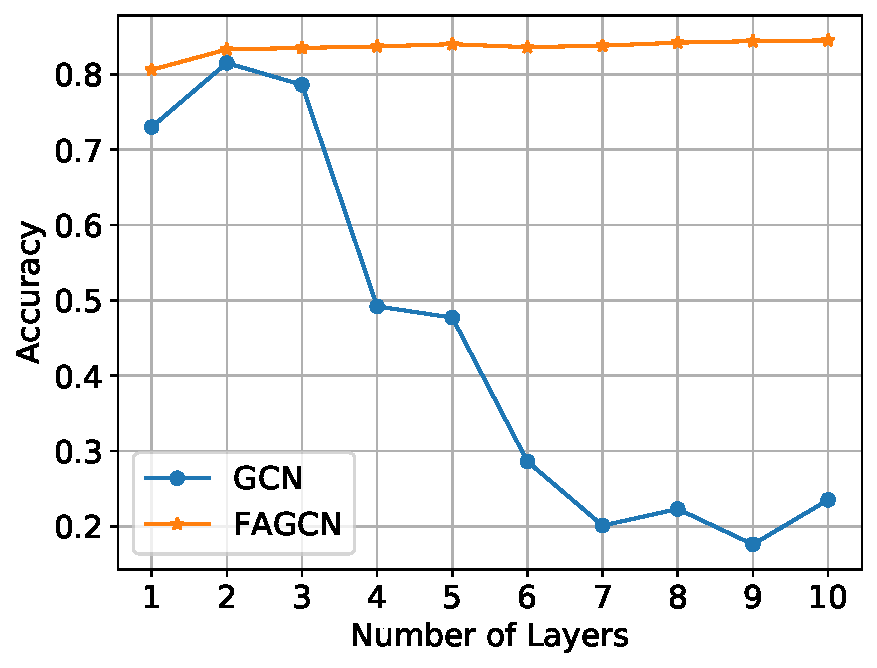
\includegraphics[width=0.45\linewidth]{image/cora_over}
        \label{cora_o}
    }
	\subfigure[Citeseer]{
        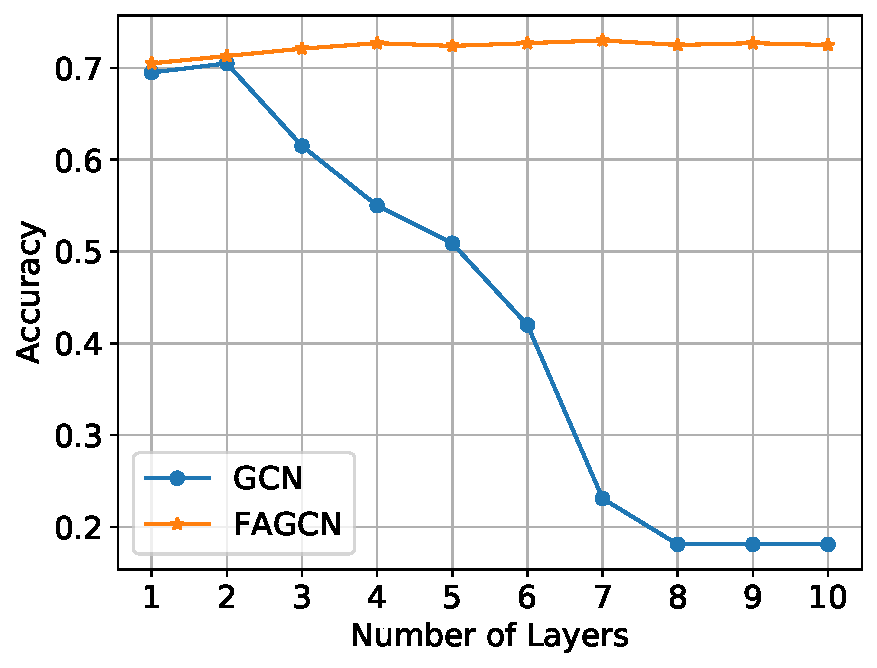
\includegraphics[width=0.45\linewidth]{image/citeseer_over}
        \label{citeseer_o}
    }
    \quad    % \quad
    \subfigure[Pubmed]{
        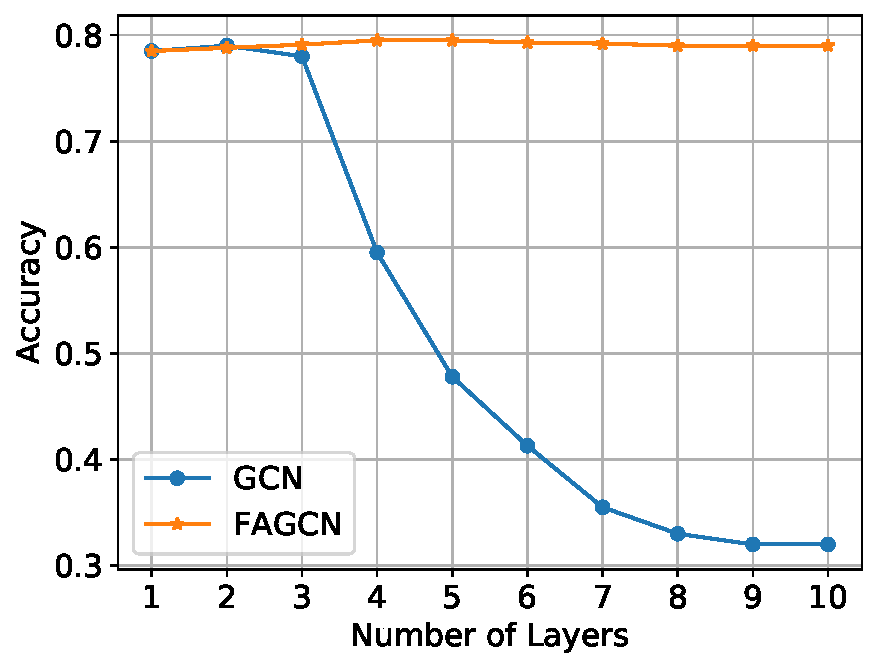
\includegraphics[width=0.45\linewidth]{image/pubmed_over}
    }
	\subfigure[Chameleon]{
        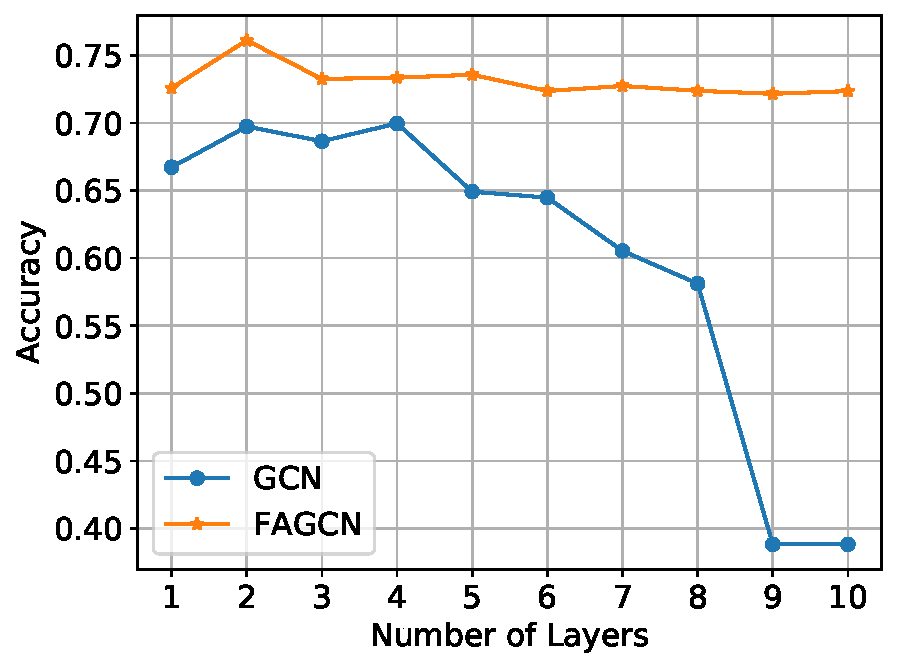
\includegraphics[width=0.45\linewidth]{image/chameleon_over}
    }
    \quad    % \quad
	\subfigure[Squirrel]{
        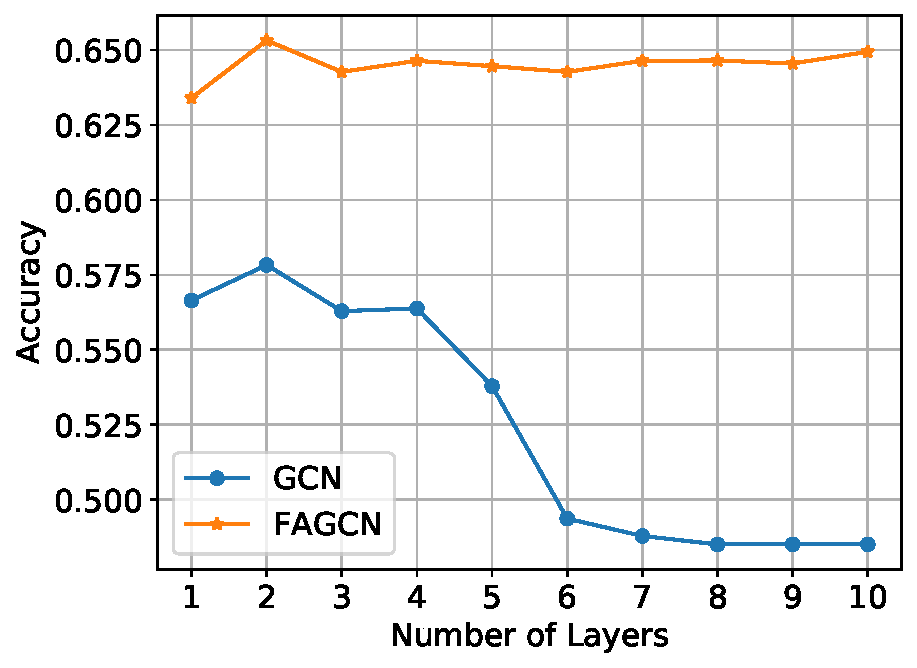
\includegraphics[width=0.45\linewidth]{image/squirrel_over}
    }
	\subfigure[Actor]{
        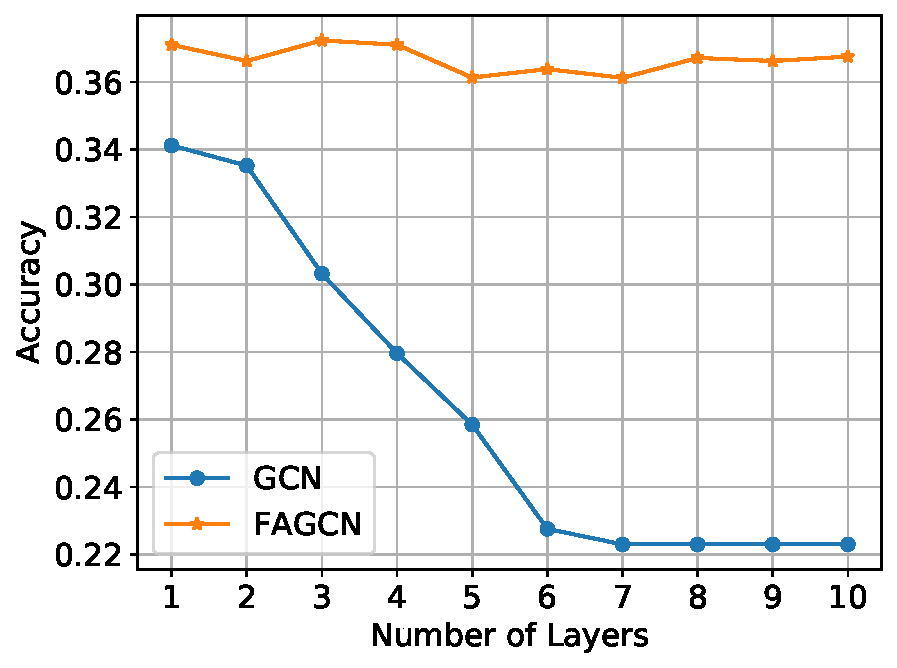
\includegraphics[width=0.45\linewidth]{image/actor_over}
    }
    \caption{Classification accuracy with different model depth.}
    \label{over-smoothing}
\end{figure}

\begin{figure*}[t]
\centering
\subfigure[Cora, Citeseer and Pubmed]{
\label{cora_h}
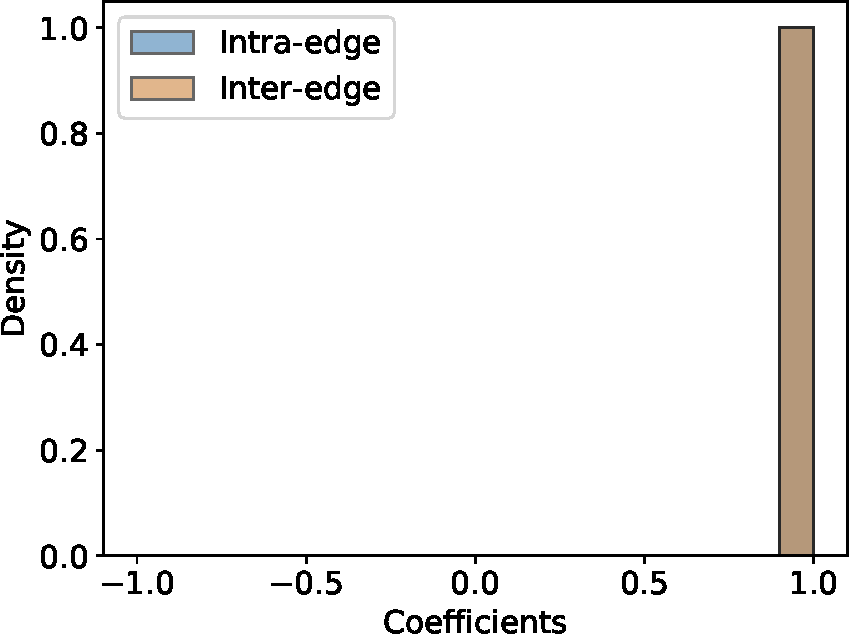
\includegraphics[width=0.23\textwidth]{image/cora_hist}
}
\subfigure[Chameleon]{
\label{chameleon_h}
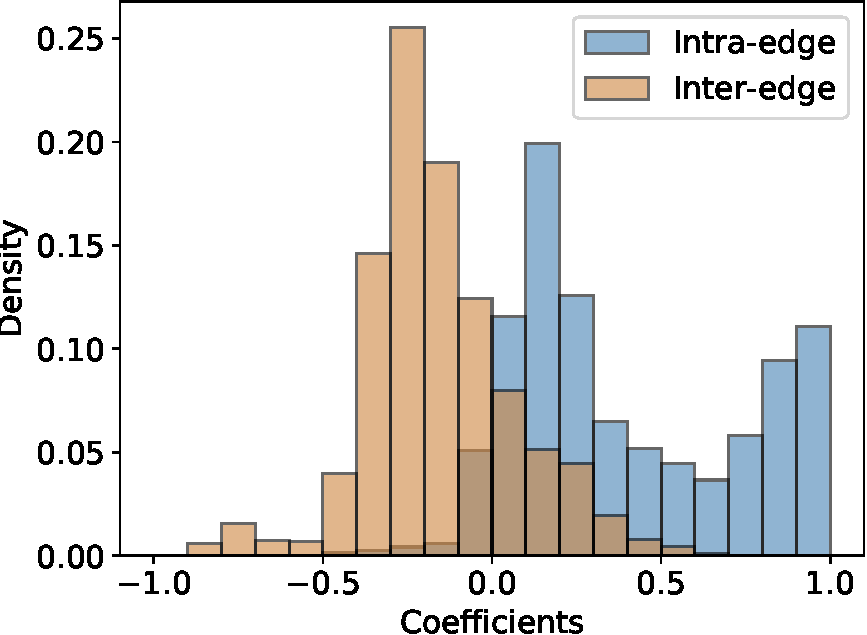
\includegraphics[width=0.23\textwidth]{image/chameleon_hist}
}
\subfigure[Squirrel]{
\label{squirrel_h}
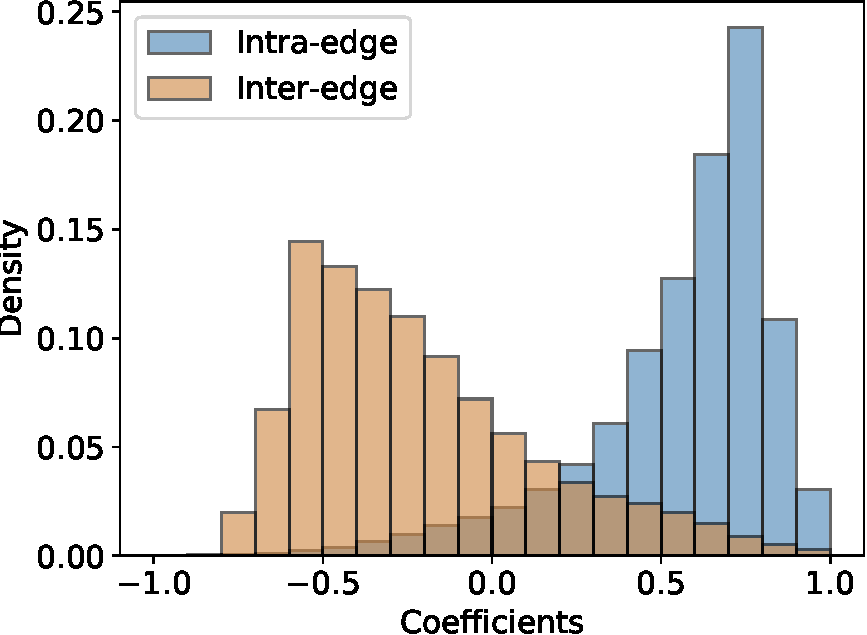
\includegraphics[width=0.23\textwidth]{image/squirrel_hist}
}
\subfigure[Actor]{
\label{film_h}
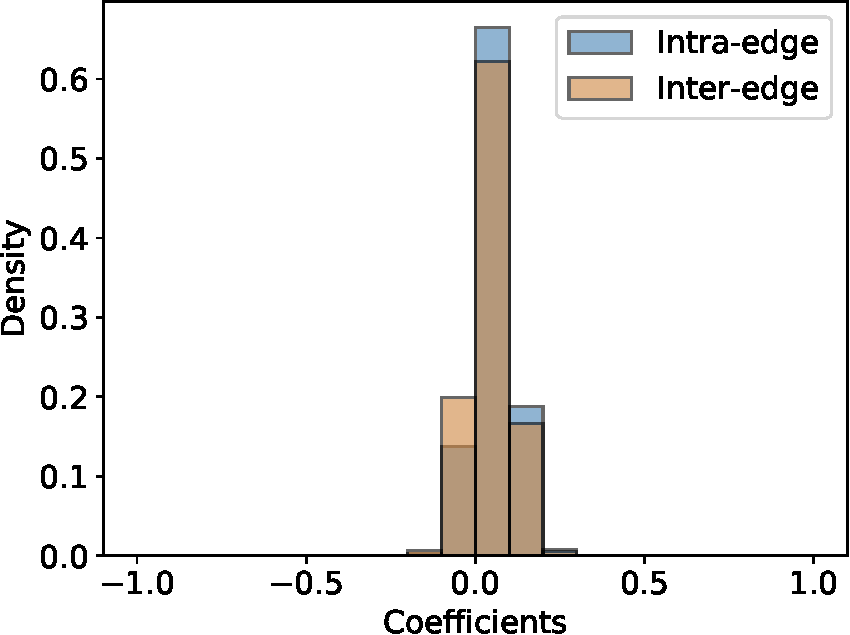
\includegraphics[width=0.23\textwidth]{image/film_hist}
}
\caption{Visualization of edge coefficients on different networks.}
\label{hist}
\end{figure*}

The performance of different methods on assortative networks is summarized in Table \ref{assortative}. GraphHeat designs a low-pass filer through heat kernel, which can better capture the low-frequency information than GCN \cite{GraphHeat}. Therefore, it performs best in the baselines. But we can see that FAGCN exceed the benchmarks on most networks due to the enhanced low-pass filter, which validates the importance of low-pass filters in the assortative networks.

Besides, the performance on disassortative networks is illustrated in Fig. \ref{disassortative}. Note that we do not choose all baselines because the methods focus on low-pass filtering have poor performance, and we use GCN and GAT as representatives. In addition, APPNP leverages residual connection to preserve the information of raw features, ChebNet uses ChebNet polynomials to approximate arbitrary convolution kernels and Geom-GCN is the state-of-the-art on disassortative networks. Therefore, comparing FAGCN with these baselines can reflect the superiority of FAGCN. From Fig. \ref{disassortative}, we can see that GCN and GAT perform worse than other methods, which indicates that only using low-pass filters is not suitable for disassortative networks. APPNP and ChebNet perform better than GCN and GAT, which shows that the raw features and polynomials can preserve the high-frequency information to some extent. Finally, FAGCN performs best in most datasets and label rates, which reflects the superiority of our method.

%In general, the results of FAGCN exceed most benchmarks, especially on the disassortative networks. We can see that most GNNs only perform well on the assortative networks, but on the disassortative network, their performance drops quickly. The reason why FAGCN performs not good on Citeseer is that there are many isolated nodes, reducing the performance of filtering. The performance of ChebNet and APPNP is better than other baselines. ChebNet uses Laplacian matrix polynomials to approximate convolution kernels.

%However, it suffers from high computations. APPNP leverages residual connection to preserve the information of raw features, but it uses a fixed ratio for each node, which is not flexible enough. It is worth noting that although ChebNet and APPNP indirectly consider the high-frequency information, they do not make full use of it. Therefore, their performance is still not as good as FAGCN. However, it suffers from high computations. APPNP leverages residual connection to preserve the information of raw features, but it uses a fixed ratio for each node, which is not flexible enough. It is worth noting that although ChebNet and APPNP indirectly consider the high-frequency information, they do not make full use of it. Therefore, their performance is still not as good as FAGCN.

%\subsection{Classification accuracy on nodes with different assortativity}

%\begin{figure}
%\centering
%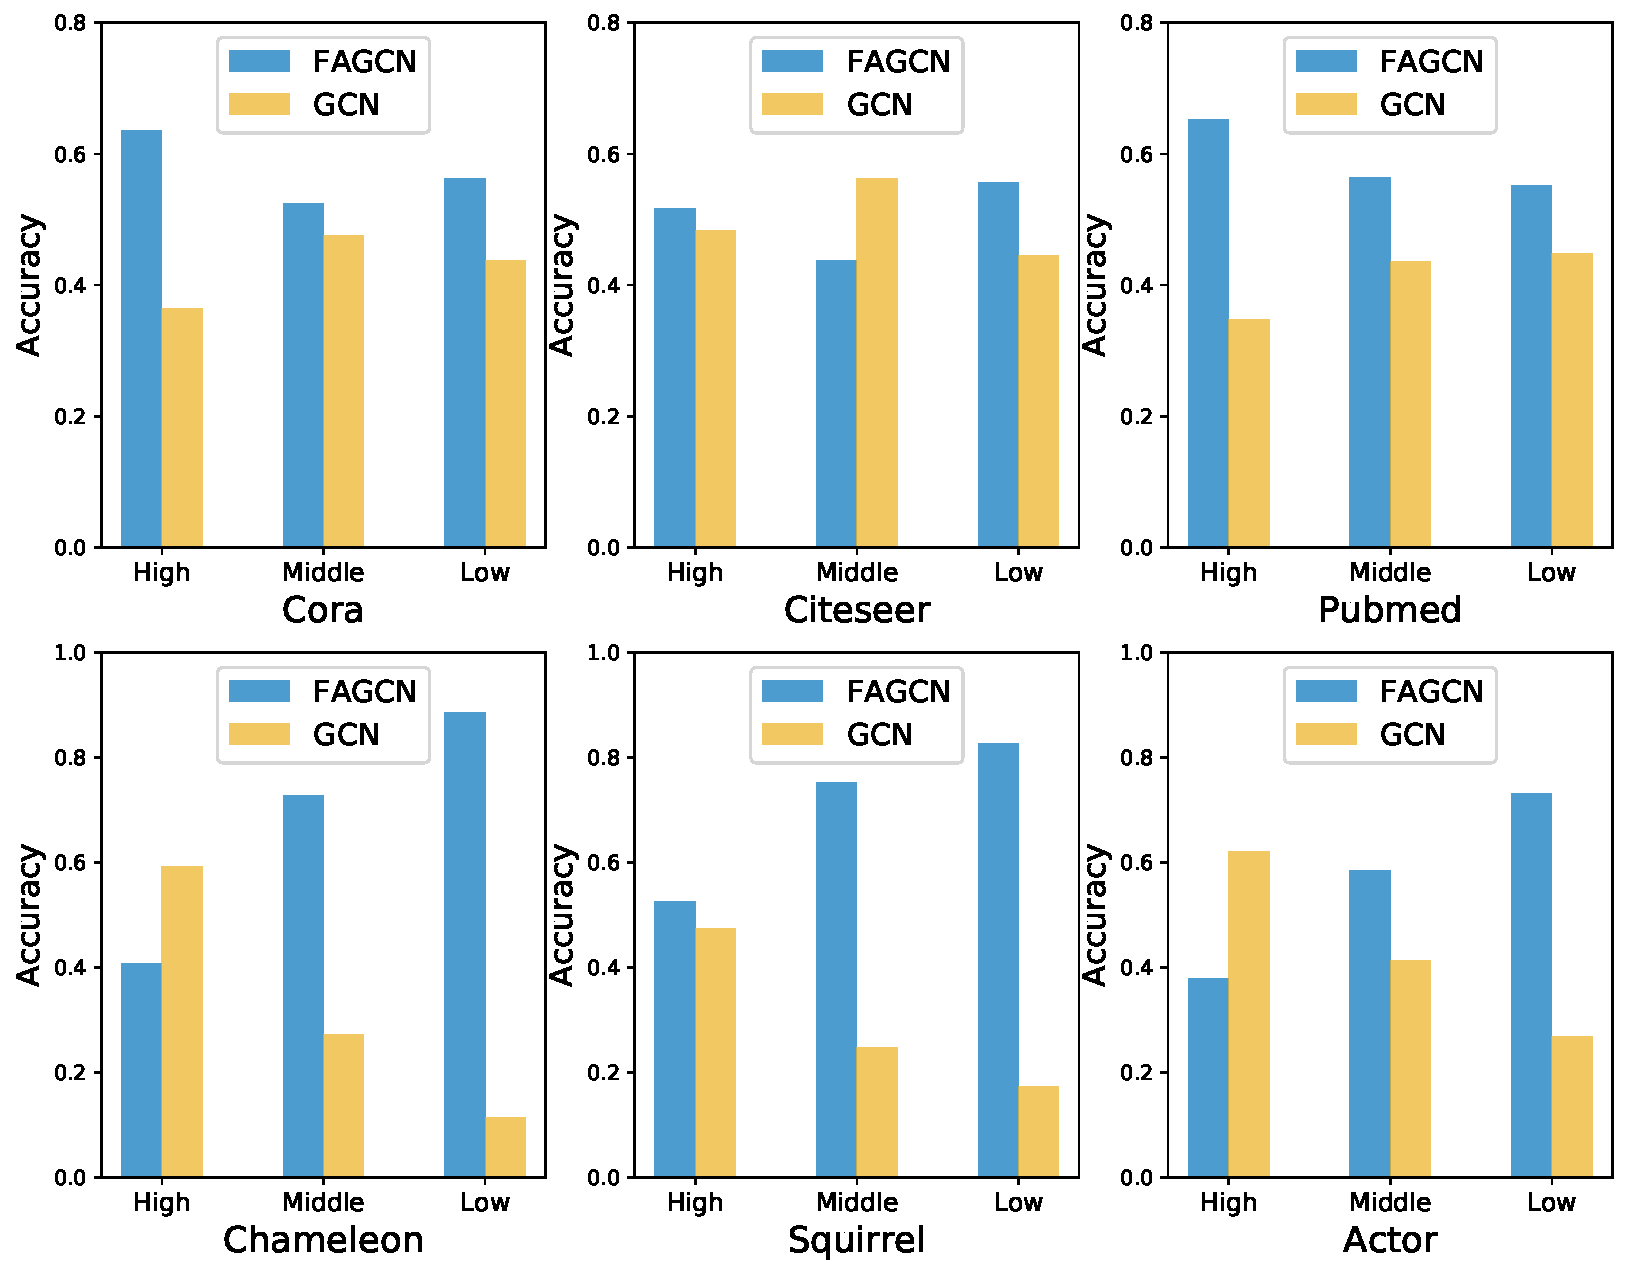
\includegraphics[width=\linewidth]{image/hetero_node}
%\caption{In each dataset, from left to right, three histograms illustrate the accuracies on High-, Middle-, Low-level assortative nodes. The blue and yellow histograms represent the accuracy of FAGCN and GCN, respectively.}
%\end{figure}

%Here we closely examine the classification performance on the nodes with different assortativity in a network. Specifically, we use the ratio of intra-connections and all connections to represent the assortativity of each node. A higher value means a more obvious assortativity.
%Then we divide the nodes into three categories based on their assortativity: Low $\in [0, \frac{1}{3})$, Middle $\in [\frac{1}{3}, \frac{2}{3}]$ and High $\in (\frac{2}{3}, 1]$.
%For a clearer comparison, we remove the nodes that are correctly classified or incorrectly classified by both methods and calculate the accuracy of GCN and FAGCN based on the remaining nodes. The results are shown in Figure \ref{hetero_node}.
%We can see that the improvement of FAGCN against GCN is obvious.
%Specifically, in assortative datasets, the improvements of FAGCN mainly focus on High-level assortative nodes.
%Because the High-level assortative nodes account for a large proportion.
%%The reasons are two-fold: One is that High-level assortative nodes account for a large proportion. Another is that most of the labeled nodes are Low-level assortative, making the prediction of other types of nodes difficult.
%In disassortative datasets, the performance of FAGCN is much better than GCN on the Middle- and Low-level assortative nodes, which proves that FAGCN has the ability to distinguish both the assortative and disassortative nodes.
%While GCN pays more attentions to the assortative nodes, which may cause a bias in the classification results.

\subsection{Alleviating Over-smoothing Problem}
To validate whether FAGCN can alleviate the over-smoothing problem, we compare the performance of GCN and FAGCN under different model depth. The results are shown in Fig. \ref{over-smoothing}. It can be seen that GCN achieves the best performance at two layers. As the number of layers increases, the performance of GCN drops rapidly, which indicates that GCN suffers from over-smoothing seriously. Instead, the results of FAGCN are stable and significantly higher than GCN on different types of networks. The reasons are two-folds: one is that in Section \ref{sec:expressive} we show that negative weights can prevents node representations from being too similar, which benefits deeper network architecture. Another is that we add the raw features, containing both low-frequency and high-frequency information, to each layer, which further keeps node representations from becoming indistinguishable. Through these two designs, when the model going deep, the performance of FAGCN is significantly better than GCN, which indicates that FAGCN has a good capability to alleviate over-smoothing.

%In particular, Fig. \ref{cora_o} and Fig. \ref{citeseer_o} illustrate that the performance of FAGCN increases as the number of layers increases, which shows that FAGCN can get more information from a larger receptive field. When the model going deep, the performance of FAGCN is significantly better than GCN, which indicates that FAGCN has a good capability to alleviate over-smoothing.

%In order to verify that FAGCN can distinguish whether two connected nodes are from the same class or not, we visualize the coefficients $\alpha_{ij}^{G}$, extracted from the first layer of FAGCN. Specially, we divide $\alpha_{ij}^{G}$ into $\alpha^{L}_{ij}$ and $\alpha^{H}_{ij}$, which represent the proportions of low-frequency and high-frequency signals, respectively. In Figure \ref{visualization}, we use box plot to show the proportions of low-frequency and high-frequency signals. We can find that when networks exhibit assortativity, $\alpha_{ij}^{L} \approx 1$ ($\alpha_{ij}^{G} \approx 1$), while when networks exhibit disassortativity, $\alpha_{ij}^{H} \approx 1$ ($\alpha_{ij}^{G} \approx -1$). Hence, the correctness of Hypothesis \ref{hypo} is verified. Besides, there are some outliers in the plot, which represent the inter-connections in assortative networks and intra-connections in disassortative networks.
%In summary, FAGCN has the ability to distinguish whether two connected nodes are from the same class.

\subsection{Visualization of Edge Coefficients}
\label{visualexperiment}

In order to verify whether FAGCN can learn different edge coefficients to adapt to different networks, we visualize the coefficients $\alpha_{ij}^{G}$, extracted from the last layer of FAGCN.
Specifically, we divide the edges into intra-edges and inter-edges based on whether two connected nodes have the same label.
It can be seen from Fig. \ref{cora_h} that in the networks with large assortativity, i.e., Cora, Citeseer and Pubmed, all edges are concentrated at the positive weights, which implies that the low-pass filter plays a major role in classification.
However, in Fig. \ref{chameleon_h} and \ref{squirrel_h}, a lot of inter-edges are distributed in negative weights, which shows that in the network with small assortativity, the high-frequency signal plays an important role in node classification.
Moreover, there is an interesting phenomenon that in Fig. \ref{film_h} the coefficients of edges are concentrated at zero. One possible reason is that the assortativity of Actor is quite small, which implies that the structures contributes less to the results of node classification, instead, the raw features dominate the classification results.
%Through these figures, we can see that FAGCN can choose different signals flexibly, without knowing the assortativity of network.

%we divide $\alpha_{ij}^{G}$ into $\alpha^{L}_{ij}$ and $\alpha^{H}_{ij}$, which represent the proportions of low-frequency and high-frequency signals, respectively. In Figure \ref{visualization}, we use box plot to show the proportions of low-frequency and high-frequency signals. We can find that when networks exhibit assortativity, $\alpha_{ij}^{L} \approx 1$ ($\alpha_{ij}^{G} \approx 1$), while when networks exhibit disassortativity, $\alpha_{ij}^{H} \approx 1$ ($\alpha_{ij}^{G} \approx -1$). Hence, the correctness of Hypothesis \ref{hypo} is verified. Besides, there are some outliers in the plot, which represent the inter-connections in assortative networks and intra-connections in disassortative networks. In summary, FAGCN has the ability to distinguish whether two connected nodes are from the same class.


\subsection{Details of Wikipedia Networks}

In this section, we aim to give more details of Wikipedia networks. First of all, Chameleon and Squirrel were originally collected for regression task, i.e., traffic prediction \cite{wikinet}. We divide the traffic into three categories: \emph{less than 1000}, \emph{between 1000 and 10000} and \emph{more than 10000}, so that they can be applied to node classification task. Secondly, labels of Chameleon and Squirrel are different from those in Geom-GCN. The reason is that in the disassortative networks provided by \cite{GeomGCN}, i.e., Cham-5 and Squi-5 in Table \ref{tab:compare}, we find that GCN performs much better than MLP. This is a strange phenomenon, because MLP uses raw features as input, which contains high-frequency information, so its performance should be better than GCN \cite{H2GNN}. Therefore, we redivide the labels based on traffic, i.e., Cham-3 and Squi-3 in Table \ref{tab:compare}, where the performance of GCN and MLP is more reasonable. Besides, we can see that FAGCN perform best on all four datasets, so its effectiveness is still guaranteed across different datasets.

%\myworries{Because MLP can be seen as an all-pass filter, containing high-frequency information, so its performance should be better than GCN. But the experimental results are contrary to the theory. This is a strange phenomenon and we leave this as a further work.}


\begin{table}[t]
  \centering
  \caption{Classification accuracy with different label division.}
    \begin{tabular}{lrrrr}
    \toprule
    \multirow{2}[4]{*}{\textbf{Method}} & \multicolumn{2}{c}{This paper} & \multicolumn{2}{c}{\cite{GeomGCN}} \\
\cmidrule(lr){2-3} \cmidrule(lr){4-5}          & \multicolumn{1}{c}{\textbf{Cham-3}} & \multicolumn{1}{c}{\textbf{Squi-3}} & \multicolumn{1}{c}{\textbf{Cham-5}} & \multicolumn{1}{c}{\textbf{Squi-5}} \\
    \midrule
    FAGCN		& \textbf{76.1\%} & \textbf{66.7\%} & \textbf{61.7\%} & \textbf{39.7\%} \\
    Geom-GCN	& 73.2\% & 63.3\% & 60.9\% & 38.1\% \\
    \midrule
    GCN   		& 72.3\% & 61.9\% & \textbf{59.8\%} & \textbf{36.9\%} \\
    MLP   		& \textbf{74.3\%} & \textbf{63.1\%} & 46.4\% & 29.7\% \\
    \bottomrule
    \end{tabular}
  \label{tab:compare}
\end{table}


\section{Related Work}

%In this section, we introduce the relevant GNN models. Specially, we divide them into two categories: spectral methods and spatial methods.

%\subsection{Spectral Graph Neural Networks}
\textbf{Spectral Graph Neural Networks.} Spectral GNNs aim to define the convolution kernel in spectral domain, by leveraging the theory of graph signal processing. Spectral CNN \cite{SpectralCNN} treats the convolution kernel as a trainable diagonal matrix and directly learns the amplitudes of signals. However, it requires the decomposition of Laplacian matrix, which is inefficient. To deal with this problem, ChebNet \cite{ChebNet} uses the polynomial of Laplacian matrix to approximate the convolution kernel and make better performance. GCN \cite{GCN} is the first-order approximation of ChebNet with a self-loop mechanism. GraphHeat\cite{GraphHeat} designs a more powerful low-pass filter through heat kernel. Besides, GWNN \cite{GWNN} replaces the eigenvectors with wavelet bases so as to further improve the efficiency of the model. Generally, spectral methods have good interpretability for the signal processing on graph, but lack generalization \cite{GraphSAGE}.

%\subsection{Spatial Graph Neural Networks}
\textbf{Spatial Graph Neural Networks.} Spatial GNNs focus on the design of aggregation function. GraphSAGE \cite{GraphSAGE} designs a permutation-invariant aggregator for message passing; GAT \cite{GAT} employs self-attention to calculate the coefficients of neighbors in aggregation; MoNet \cite{MoNet} provides a unified generalization of graph convolutional architectures in spatial domain; PPNP \cite{PPNP} incorporates personalized PageRank to the aggregation function;
Geom-GCN \cite{GeomGCN} utilizes the structural similarity to capture the long-range dependencies in disassortative graphs.
H2GNN \cite{H2GNN} separates the raw features and aggregated features so as to preserve both high-frequency and low-frequency information, but it lacks adaptability;
Non-Local GNN \cite{Non-Local} designs an attention-guided sorting mechanism to transform the disassortative networks into assortative networks, which costs a lot of computations.
Generally, spatial methods are more flexible and scalable, but lack interpretability.
It is worth noting that FAGCN is a spatial method, but it still has good interpretability, which combines the advantages of both spectral and spatial methods.

\section{Conclusion}

In this paper, we make the attempt to study the roles of low-frequency and high-frequency signals in GNNs and show that both of them are helpful in learning node representations. Based on this observation, we design a novel frequency adaptation graph convolutional network to adaptively combine the low-frequency and high-frequency signals. Theoretical analysis shows that the expressive power of our model is greater than most existing GNNs.
An important direction of future work is to use more signals with different frequencies, e.g., the intermediate frequency signals.

\section{Acknowledgments}
This work is supported in part by the National Natural Science Foundation of China (No. U1936220, U1936104, 61772082, 61702296, 62002029, 61972442), Meituan-Dianping Group and BUPT Excellent Ph.D. Students Foundation (No. CX2020115). Huawei Shen is funded by Beijing Academy of Artificial Intelligence (BAAI).


% \bibliographystyle{aaai}
Eligendi error reprehenderit repellat modi animi praesentium, recusandae esse dolorem ipsam explicabo eligendi error quae repellat hic tempora consequatur, dolorem natus temporibus rem voluptatum sapiente?Reiciendis libero eaque perspiciatis esse debitis quo distinctio quasi
\bibliography{FAGCN}

\end{document}